\documentclass{beamer}
\usetheme{CambridgeUS} % My favorite!
\setbeamercolor{title}{fg=red!80!black,bg=white!90!black}
\newenvironment{conenv}{\only{\setbeamercolor{local structure}{fg=darkred}}}{}
\setbeamercovered{dynamic}
\setbeamertemplate{navigation symbols}{} 
\definecolor{links}{HTML}{2A1B81}
%\hypersetup{colorlinks,linkcolor=,urlcolor=links}
\hypersetup{colorlinks,linkcolor=,urlcolor=blue!70!black}
%\hypersetup{colorlinks,linkcolor=,urlcolor=red!80!black}
\usepackage[utf8]{inputenc}
\usepackage{eurosym}
\usepackage{color}
\usepackage{multirow}
\usepackage{hhline}
\usepackage{amsmath}
\usepackage{fancybox}
%\usepackage{kpfonts}
\usepackage[framemethod=TikZ]{mdframed}
\usepackage{tikz}
\usetikzlibrary{backgrounds}
\usepackage{rotating}
\usepackage[skins]{tcolorbox}
\usepackage[percent]{overpic}
\mathchardef\mhyphen="2D
\setbeamerfont{page number in head/foot}{size=\tiny \bf}
\setbeamercolor{page number in head/foot}{fg=red!80!black}
\setbeamerfont{frametitle}{size=\footnotesize}
%\setbeamertemplate{footline}[frame number]
\usepackage{appendixnumberbeamer}
\usepackage{bbding}
\usepackage{pifont}
\usepackage{graphicx}
\usepackage{booktabs}
\usepackage{array}
\usepackage{calc}
\usepackage{makecell}
\newcommand<>{\superimpose}[2][]{%
    \tikz[overlay, remember picture]{%
        \filldraw#3[fill=white, opacity=0.8] (current page.north west) rectangle (current page.south east);
        %\filldraw#3[fill=white, opacity=0.8] (accent_left.south east) rectangle (current page.south east);
        \node#3[at=(current page.center), rotate =20,line width=0.3mm, #1]
			{\vspace{35pt} #2 \vspace{35pt}};
    }%
}
\newcolumntype{P}[1]{>{\centering\arraybackslash}p{#1}}

\settowidth{\leftmargini}{\usebeamertemplate{itemize item}}
\addtolength{\leftmargini}{\labelsep}    % to move bullets

\addtolength{\textwidth}{0cm}
\DeclareRobustCommand{\frac}[3][0pt]{%
  {\begingroup\hspace{#1}#2\hspace{#1}\endgroup\over\hspace{#1}#3\hspace{#1}}}
%\addtolength{\hoffset}{-4cm}

%General
\newcommand{\breakhere}{\noindent\rule{15cm}{0.4pt}}
\newcommand{\qm}{\textbf{\textcolor{red}{?}}}
\newcommand*\plus{\ensuremath{\texttt{+}}~}
\newcommand*\plusn{\ensuremath{\texttt{+}}}
\newcommand*\hy{\ensuremath{\mbox{-}}}

% Chapter 4
\providecommand{\httwo}{\ensuremath{H_{\mathrm{T,2}}/2}\xspace}
\providecommand{\ptone}{\ensuremath{p_{\mathrm{T,1}}}\xspace}
\providecommand{\pttwo}{\ensuremath{p_{\mathrm{T,2}}}\xspace}
\providecommand{\cme}{$\sqrt{s}$\xspace}
\providecommand{\MadGraphF}{{\textsc{MadGraph5}}\xspace}






% Itemize
\newcommand*\ball{\setbeamertemplate{itemize items}[ball]}
\newcommand*\cir{\setbeamertemplate{itemize items}[circle]}
\newcommand*\tri{\setbeamertemplate{itemize items}[triangle]}

%Colors
%\newcommand*\mycolor{\textcolor{red!80!black}}
%\newcommand*\blue{\textcolor{blue!70!black}}
%\newcommand*\green{\textcolor{green!50!black}}
%\definecolor{auburn}{rgb}{0.07, 0.04, 0.56}
\newcommand*\AN{\textcolor{auburn}}
\newcommand*\yes{\textcolor{red!80!black} {\Checkmark }}
\newcommand*\no{\textcolor{red!80!black} {\XSolidBrush}}
%\definecolor{pink}{rgb}{1.0, 0.11, 0.81}
%spaces
\newcommand{\tab}[1]{\hspace{.2\textwidth}\rlap{#1}}
\newcommand{\itab}[1]{\hspace{.12\textwidth}\rlap{#1}}
%\tcbset{colframe=white,colback=white,nobeforeafter}
\newcommand{\mybox}[2]{{\color{red!80!black}\fbox{\normalcolor#2}}}
\setlength\fboxrule{0.8pt}
%Def
\newcommand{\lumins}{\ensuremath{\mathcal{L}}}

\providecommand{\ptave}{\ensuremath{\langle p_\mathrm{T1,2}\rangle}\xspace}
\providecommand{\bqm}{\ensuremath{\scalebox{1.2}{\textbf{?}}}\xspace}
\providecommand{\RooUnfold} {{\textsc{RooUnfold}}\xspace}
\providecommand{\refe}{\ensuremath{\textcolor{red!80!black}{\bf [REF]}}\xspace}
\providecommand{\HERWIGPP} {{\textsc{herwig++}}\xspace}
\providecommand{\PYTHIAS} {{\textsc{pythia6}}\xspace}
\providecommand{\PYTHIAE} {{\textsc{pythia8}}\xspace}
\providecommand{\POWHEG} {{\textsc{powheg}}\xspace}
\providecommand{\NLOJETPP} {{\textsc{NLOJet++}}\xspace}
\providecommand{\RunDec}{{\textsc{RunDec}}\xspace}
\providecommand{\fastNLO} {{\textsc{fastNLO}}\xspace}
\providecommand{\fastjet} {{\textsc{FastJet}}\xspace}
\providecommand{\mur}{\ensuremath{\mu_r}\xspace}
\providecommand{\muf}{\ensuremath{\mu_f}\xspace}
\providecommand{\alpsmz}{\ensuremath{\alpha_s(M_Z)}\xspace}
\providecommand{\chisq}{\ensuremath{\chi^2}\xspace}
\providecommand{\chisqndof}{\ensuremath{\chi^2/n_\mathrm{dof}}\xspace}
\providecommand{\alps}{\ensuremath{\alpha_S}\xspace}
\providecommand{\alpsmusq}{\ensuremath{\alpha_S(\mu_r^2)}\xspace}
\providecommand{\alpsmzsq}{\ensuremath{\alpha_S(M_Z^2)}\xspace}
\providecommand{\alpsqsq}{\ensuremath{\alpha_S(Q^2)}\xspace}
\providecommand{\alpsmu}{\ensuremath{\alpha_S(\mu_r)}\xspace}
\providecommand{\alpsmz}{\ensuremath{\alpha_S(M_Z)}\xspace}
\providecommand{\alpsq}{\ensuremath{\alpha_S(Q)}\xspace}
\providecommand{\ratio}{\ensuremath{R_{32}}\xspace}
\providecommand{\LHAPDF}{{\textsc{LHAPDF}}\xspace}
\providecommand{\LHAPDFS}{{\textsc{LHAPDF6}}\xspace}
\providecommand{\NF}{\ensuremath{N_F}\xspace}
\providecommand{\Ztwostar}{\ensuremath{\mathrm{Z2}^\star}\xspace}
\newcommand{\hftwo}{\hspace*{\fill}}
\newcommand{\rbthm}{\rule[-2ex]{0ex}{5ex}}
\newcommand{\rbtrr}{\rule[-0.8ex]{0ex}{3.2ex}}
\newcommand*\alpsmzns{\ensuremath{\alpha_S(M_Z)}}
\newcommand*\alpsns{\ensuremath{\alpha_S}}
\newcommand*\httwons{\ensuremath{\mathrm{H_{T,2}}/2}}
\newcommand*\ptavens{\ensuremath{\mathrm{\langle p_\mathrm{T_{1,2}}\rangle}}}
\newcommand*\rations{\ensuremath{\mathrm{R_{32}}}}

\newcommand*\pas{\includegraphics[scale=0.3]{/home/anter/Desktop/Analysis_8/Present_Latex/Pre-approval/Plots/pas_new.png}}
\newcommand*\staru{\ensuremath{\blue{^{*}}}}
\newcommand*\unc{\ensuremath{\blue{^{\#}}}}
\newcommand*\pts{p$^2_{\mathrm{T}}$}
\newcommand*\msd{m$_{\mathrm{SD}}$}
\newcommand*\msds{m$^2_{\mathrm{SD}}$}
\newcommand*\met{E$\mathrm{_{T}^{miss}}$}
\newcommand*\varnd{$\mathrm{N_{2,DDT}^1}$}
\newcommand*\vartau{$\mathrm{\tau_{21}^{DDT}}$}
\newcommand*\varn{$\mathrm{N_{2}^1}$}
\newcommand*\rapa{$\mathrm{|\eta|}$}
\newcommand*\gr{$\mathrm{>}~$}
\newcommand*\ls{$\mathrm{<}~$}
\newcommand{\inv}{$^{\text{-}1}$}



\vspace{15 mm}

\title[Multijet Cross-Section Ratios(Ph.D. Defense)] {\normalsize MEASUREMENT OF MULTIJET CROSS-SECTION RATIOS \\IN PROTON-PROTON COLLISIONS WITH THE CMS \\DETECTOR AT THE LHC}

\author[Anterpreet Kaur]{\blue{Anterpreet Kaur} \\ { \normalsize Supervisor : Prof. Manjit Kaur}\\}
\vspace{-3mm}
\institute[]
{
%{ \normalsize \blue{Supervisor : Prof. Manjit Kaur }}\\
% \medskip
 %\medskip
 %\medskip
 %\medskip
 Department of Physics \\ Panjab University \\ Chandigarh, India
}
\date[October, 2018]{\footnotesize \textcolor{blue!0!black}{}}

\begin{document}
\setbeamercolor{item}{fg=red!70!black}
\setbeamertemplate{enumerate items}[default]

%###################################### Slide : 1 ######################################
\begin{frame}[plain]
\vspace{0.50mm}
\includegraphics[scale = 0.18]{/home/anter/Desktop/Analysis_8/Present_Latex/Klaus/plots/cms.jpeg}
\hfill
\hspace{50 mm}
\includegraphics[scale = 0.20]{/home/anter/Desktop/Analysis_8/Present_Latex/Klaus/plots/pu.png}
\vspace{0.2mm}
\titlepage
\vspace{2.2mm}
\begin{beamercolorbox}[wd=120mm,ht=1.5mm,center,shadow=true, rounded=true]{redgrey}
{}
{\scriptsize \mycolor{Ph.D. Defense \hfill \hspace{75mm} October , 2018}}
\end{beamercolorbox}
\end{frame}

%###################################### Slide : 2 ######################################
\begin{frame}
\frametitle{\centerline{Outline}}
\setlength\labelsep {\dimexpr\labelsep + 0.05em\relax}
\setlength\leftmargini{\dimexpr\leftmargini + 0.05em\relax}
\begin{itemize}
\item {\scriptsize Motivation
\vspace{1mm}
\item CMS detector
\vspace{1mm}
\item Analysis Strategy
\vspace{1mm}
\item Measurement of inclusive multijet cross-sections
\vspace{1mm}
\item Theoretical Predictions
\vspace{1mm}
\item Data-Theory Comparisons
\vspace{1mm}
\item Cross-section Ratio R$_{32}$
\vspace{1mm}
\item Determination of the Strong Coupling Constant, \alpsmz
\vspace{1mm}
\item Summary and Outlook \\}
\end{itemize}
\begin{comment}
\begin{itemize}
\tri
\item {\scriptsize Datasets \& Monte-Carlo (MC) Samples
\vspace{1mm}
\item Trigger Studies
\vspace{1mm}
\item Event Selection
\vspace{1mm}
\item Detector Level Comparisons
\vspace{0.5mm}

\item Measurement of inclusive multijet cross-sections
\vspace{0.5mm}
\begin{comment}\cir
\begin{itemize}
{\scriptsize \item Jet Energy Resolution (JER) 
\vspace{1mm}
\item Closure tests and Unfolding
\vspace{1mm}
\item Experimental Uncertainties  \\ } 
\end{itemize} 
\tri
\item {\scriptsize  Theoretical Predictions \\}
\vspace{0.5mm}
\cir
\begin{itemize}
{\scriptsize \item Non-perturbative Corrections 
\vspace{1mm}
\item Electroweak Corrections
\vspace{1mm}
\item Theoretical Uncertainties \\}
\end{itemize}
\tri
\vspace{1mm}
\item {\scriptsize  Data-Theory Comparisons
\vspace{1mm}
\item Cross-section Ratio R$_{32}$
\vspace{1mm}
\item Determination of the Strong Coupling Constant, \alpsmz }
\vspace{1mm}
\end{itemize}
\item {\scriptsize Summary and Outlook\\}
\end{itemize}
\end{comment}
\end{frame}

%###################################### Slide : 2 ######################################
\begin{frame}
\frametitle{\centerline{Introduction}}
\setlength\labelsep {\dimexpr\labelsep + 0.05em\relax}
\setlength\leftmargini{\dimexpr\leftmargini + 0.05em\relax}
\hspace*{2mm}\begin{minipage}[thbp]{0.6\textwidth}
\vspace{1mm}
\hspace*{-4mm}\blue{\bf \footnotesize Jets : \\}
\vspace{-4mm}
\begin{itemize}
\item {\scriptsize key component to extend our understanding of the Standard Model physics
\vspace{1mm}
\item signatures of large momentum transfers at short distances, belong primarily to perturbative domain of Quantum Chromodynamics (pQCD)
\vspace{1mm}
\item produced abundantly in the collisions of protons at the Large Hadron Collider (LHC)
\vspace{1mm}
%\item provide an excellent opportunity for testing the predictions of pQCD at high energies 
\item important backgrounds for many new physics models\\}
\end{itemize}
\end{minipage}
\hspace{0mm}
\begin{minipage}[thbp]{0.08\textwidth}
\vspace{-15mm}
\hspace{15mm}\includegraphics[scale = 0.4]{/home/anter/Desktop/DIS/Presentation/Figures/Figures_hh-collisions-pieces.png}
\end{minipage}
\hspace*{2mm}\begin{minipage}[thbp]{0.6\textwidth}
\vspace{4mm}
\hspace*{-4mm}\blue{\bf \footnotesize Inclusive jet cross section measurement : \\}  
\vspace{-4mm}
\begin{itemize}
\item {\scriptsize gives important information about the strong coupling constant \alps \\}
\vspace{-7.0mm}
\begin{align*}
\resizebox{.7\hsize}{!}{$\rm \blue{\sigma_{i\mbox{-}jet} = \sigma(pp\to i~jets~\plus X) \propto \alpsns^{i}}$}
\end{align*}
\item {\scriptsize provides a deep insight to understand the proton structure by deriving constraints on the parton distribution functions (PDFs) \\}
\end{itemize}
%\begin{itemize}
%\item {\scriptsize Jet properties such as jet shapes, mass, charge etc. : key ingredients of Standard Model (SM) physics measurements and for beyond SM physics searches \\}
%\end{itemize}
\end{minipage}
\begin{minipage}[thbp]{0.14\textwidth}
\vspace{-15.5mm}
%\vspace{-2.5mm}
\begin{overpic}[scale = 0.22]{/home/anter/Desktop/Thesis/Figures/Factorization_2.pdf}
\vspace{-4.2mm}
\put(-24,0){\tiny $\sigma_{P_1P_2 \rightarrow X} = \blue {\sum\limits_{i,j}^{}\int_{}^{} dx_1dx_2f_{i,P_1}(x_1,\muf)f_{j,P_2}(x_2,\muf)}$}
\put(10,-13){\tiny$\times~\mycolor {\hat\sigma_{ij\rightarrow X} \Bigg(x_1p_1,x_2p_2,\alpha(\mur^2),\frac{Q^2}{\muf^2}\Bigg)}$}
\end{overpic}
\end{minipage}
\end{frame}

%narrow cone of particles produced by the hadronization of quarks or gluons produced in hadron colliosns in a particle physics or heavy ion experiment

%###################################### Slide : 3 ######################################
\begin{frame}
\frametitle{\centerline{Inclusive jet production @ 8 TeV}}
\setlength\labelsep {\dimexpr\labelsep + 0.05em\relax}
\setlength\leftmargini{\dimexpr\leftmargini + 0.05em\relax}
\hspace*{2mm}\begin{minipage}[thbp]{0.55\textwidth}
%\hspace*{0mm}\begin{beamercolorbox}[wd=43mm,ht=4.5mm,center,shadow=true, rounded=true]{redgrey}
%{}
\hspace*{0mm}\begin{beamercolorbox}[wd=52mm,ht=7.0mm,center,shadow=true, rounded=true]{redgrey}
{}
{{\scriptsize \mycolor{\vspace{1mm}Double-differential cross-section }\\}
\resizebox{0.77\hsize}{!}{\mycolor{$\frac{d^2\sigma}{dp_{\rm T} dy} = \frac{1}{\epsilon~\mathcal{L}_{\mathrm{int,eff}}}\frac{N_\mathrm{jets}}{\Delta p_{\rm T} (2\Delta |y|)}$}}}
\end{beamercolorbox}\\
\vspace{-1mm}
\begin{itemize}
\item {\footnotesize Measurement at 8 TeV \\ \lumi = 19.7 \inv{fb} and \lumi = 5.6 \inv{pb}
\vspace{2mm}
\item anti-\kt jets with R = 0.7
\vspace{2mm}
\item 21 $\leq$ \ptr~\ls 74 GeV, upto $|$y$|$= 4.7
\vspace{1mm}
\item[] 74 $\leq$ \ptr~\ls 2500 GeV, upto $|$y$|$ = 3.0 
\vspace{2mm}
\item Theoretical NLO calculations : \\}
\begin{itemize}
\tri
\item {\footnotesize using CT10 PDF set
\vspace{2mm}
\item corrected for non-perturbative (NP) and electroweak (EWK) effects \\}
\end{itemize}
\ball
\end{itemize}
\end{minipage}
\hspace*{-10mm}
\begin{minipage}[thbp]{0.1\textwidth}
\vspace{13mm}
\hspace*{-4mm}\includegraphics[scale = 0.32]{/home/anter/Desktop/DIS/Presentation/Plots/CMS-SMP-14-001_Figure_003.pdf}\\ \\
\hspace*{35mm}\begin{beamercolorbox}[wd=23mm,ht=1mm,center,shadow=true, rounded=true]{redgrey}
{}
{\scalebox {0.61} {\mycolor{JHEP 03 (2017) 156}}}
\end{beamercolorbox}
\end{minipage}
\end{frame}

%###################################### Slide : 4 ######################################
\begin{frame}
\frametitle{\centerline{Inclusive jet production @ 8 TeV}}
\setlength\labelsep {\dimexpr\labelsep + 0.05em\relax}
\setlength\leftmargini{\dimexpr\leftmargini + 0.05em\relax}
\hspace*{2mm}\begin{minipage}[thbp]{0.6\textwidth}
%\begin{itemize}
%\item 
\hspace*{-4mm}\blue{\bf \scriptsize Data/theory using the CT10 NLO PDF : \\} 
\vspace*{-5mm}
\begin{itemize}
\item {\scriptsize Good agreement except low-\ptr region 
\item Data uncertainties : jet energy scale (1-45\%), \\lumi (2.6\%)
\item NLO uncertainties : scale (5-40\%), PDF (10-100\%) \\}
\end{itemize}
\hspace*{-4mm}\blue{\bf \scriptsize Ratios to CT10 PDF : \\} 
\vspace*{-5mm}
\begin{itemize}
\item {\scriptsize Significant discrepancies with ABM11 PDF \\}
%\item Differences in the high-\ptr region using different PDFs\\}
\end{itemize}
\hspace*{-4mm}\blue{\bf \scriptsize Ratios 2.76/8 TeV, 7/8 TeV : \\} 
\vspace*{-5mm}
\begin{itemize}
\item {\scriptsize Partial reduction of uncertainties $\rightarrow$ better sensitivity to PDFs\\}
\end{itemize}
\vspace*{-2mm}
\hspace*{15mm}\includegraphics[scale = 0.21]{/home/anter/Desktop/DIS/Presentation/Plots/cropped_CMS-SMP-14-001_Figure_008-a.pdf}\\
\end{minipage}
\hspace*{-2mm}
\begin{minipage}[thbp]{0.1\textwidth}
\vspace{-6mm}
\hspace*{0mm}\includegraphics[scale = 0.25]{/home/anter/Desktop/DIS/Presentation/Plots/cropped_CMS-SMP-14-001_Figure_004-a.pdf}\\
\hspace*{0mm}\includegraphics[scale = 0.25]{/home/anter/Desktop/DIS/Presentation/Plots/cropped_CMS-SMP-14-001_Figure_005-a.pdf}\\
%\hspace*{5mm}\includegraphics[scale = 0.22]{/home/anter/Desktop/DIS/Presentation/Plots/cropped_CMS-SMP-14-001_Figure_008-a.pdf}\\
\hspace*{20mm}\begin{beamercolorbox}[wd=23mm,ht=1mm,center,shadow=true, rounded=true]{redgrey}
{}
{\scalebox {0.61} {\mycolor{JHEP 03 (2017) 156}}}
\end{beamercolorbox}
\end{minipage}
\end{frame}

%###################################### Slide : 5 ######################################
\begin{frame}
\frametitle{\centerline{Inclusive jet production @ 8 TeV}}
\setlength\labelsep {\dimexpr\labelsep + 0.05em\relax}
\setlength\leftmargini{\dimexpr\leftmargini + 0.05em\relax}
\hspace*{2mm}\begin{minipage}[thbp]{0.7\textwidth}
\hspace*{-4mm}\blue{\bf \footnotesize QCD analysis using HeraFitter (1.1.1)\\}
\vspace{-4mm}
\begin{itemize}
\item {\footnotesize Inclusive cross sections \plus HERA inclusive DIS : \\}
\begin{itemize}
\tri
\item {\footnotesize probes hadronic parton-parton interaction over a \\ wide range of $x$ and $Q$ 
\vspace{1mm}
\item constraints on PDFs
\vspace{1mm}
\item significant improvement of the gluon distribution \\}
\end{itemize}
\end{itemize}
\ball
\hspace*{-4mm}\blue{\bf \footnotesize Extraction of \alps\\}
\vspace{-4mm}
\begin{itemize}
\item {\footnotesize Least square minimization on $p_{\rm T}$($y$) spectrum : \\}
\begin{itemize}
\tri
\item {\footnotesize using the CT10 NLO PDF set \\}
\end{itemize}
\vspace{-1mm}
%\hspace*{-3mm}{\scalebox {0.70} {\blue {\alpsmz = 0.1164 $^{+0.0025}_{-0.0029}$(PDF) $^{+0.0053}_{-0.0028}$(scale) $\pm$0.0001(NP) $^{+0.0014}_{-0.0015}$(exp)}}}\\	
\hspace*{15mm}{\scalebox {0.80} {\blue {\alpsmz = 0.1164 $^{+0.0060}_{-0.0043}$}}}
%\hspace*{7mm}{\scalebox {0.70} {\blue { = 0.1164 $^{+0.0060}_{-0.0043}$}}}
\vspace{1mm}
\begin{itemize}
\tri
\item {\footnotesize using the NNPDF3.0 NLO PDF set \\}
\end{itemize}
\vspace{-1mm}
\hspace*{15mm}{\scalebox {0.80} {\blue {\alpsmz = 0.1172 $^{+0.0083}_{-0.0075}$}}}
\item {\footnotesize Consistent with the world average value : \\} \vspace{1mm}\hspace*{5mm}{\scalebox {0.80} {\blue{\alpsmz = 0.1181 $\pm$ 0.0011}}}
\end{itemize}
\ball
\end{minipage}
\hspace*{-6mm}
\begin{minipage}[thbp]{0.08\textwidth}
\hspace*{0mm}\includegraphics[scale = 0.16]{/home/anter/Desktop/DIS/Presentation/Plots/cropped_CMS-SMP-14-001_Figure_015-a.pdf}\\
\hspace*{3mm}\includegraphics[scale = 0.19]{/home/anter/Desktop/DIS/Presentation/Plots/cropped_CMS-SMP-14-001_Figure_012.pdf}\\
\hspace*{12mm}\begin{beamercolorbox}[wd=23mm,ht=1mm,center,shadow=true, rounded=true]{redgrey}
{}
{\scalebox {0.61} {\mycolor{JHEP 03 (2017) 156}}}
\end{beamercolorbox}
\end{minipage}
\end{frame}

%###################################### Slide : 6 ######################################
\begin{frame}
\frametitle{\centerline{Inclusive jet production @ 13 TeV}}
\setlength\labelsep {\dimexpr\labelsep + 0.05em\relax}
\setlength\leftmargini{\dimexpr\leftmargini + 0.05em\relax}
\hspace*{2mm}\begin{minipage}[thbp]{0.6\textwidth}
\vspace{-2.5mm}
\hspace*{0mm}\begin{beamercolorbox}[wd=52mm,ht=7.0mm,center,shadow=true, rounded=true]{redgrey}
{}
{{\scriptsize \mycolor{\vspace{1mm}Double-differential cross-section }\\}
\resizebox{0.77\hsize}{!}{\mycolor{$\frac{d^2\sigma}{dp_{\rm T} dy} = \frac{1}{\epsilon~\mathcal{L}_{\mathrm{int,eff}}}\frac{N_\mathrm{j}}{\Delta p_{\rm T} \Delta y}$}}}
\end{beamercolorbox}\\
\vspace{-2mm}
\begin{itemize}
\item {\footnotesize Measurement at 13 TeV \\ \lumi = 71 \inv{pb} and \lumi = 44 \inv{pb}
\vspace{1mm}
\item anti-\kt jets with R = 0.4 and R = 0.7
\vspace{1mm}
\item \ptr \ls 2 TeV
\vspace{1mm}
\item Large rapidity coverage : $|$y$|$ \ls 3, 3.2 \ls $|$y$|$ \ls 4.7 
\vspace{1mm}
\item Theoretical NLO calculations : \\}
\begin{itemize}
\tri
\item {\footnotesize using CT14 PDF set
\vspace{2mm}
\item corrected for non-perturbative (NP) and electroweak (EWK) effects \\}
\end{itemize}
\vspace{-1mm}
\ball
\item {\footnotesize x-sections accuratey described for R = 0.7, while for R = 0.4 theory overestimates by 5–10\%\\}
%\item {\footnotesize \POWHEG\plusn \PYTHIAE~gives a good agreement in both values of R. \\}
%\item {\footnotesize PH\plusn P8 CUETM1 gives a good agreement in both values of R. \\}
\end{itemize}
\end{minipage}
\hspace{5mm}
\begin{minipage}[thbp]{0.1\textwidth}
\vspace{-1.2mm}
\includegraphics[scale = 0.195]{/home/anter/Desktop/DIS/Presentation/Plots/CMS-SMP-15-007_Figure_004-a.pdf}\\
\includegraphics[scale = 0.195]{/home/anter/Desktop/DIS/Presentation/Plots/CMS-SMP-15-007_Figure_005-b.pdf}\\
\hspace*{10mm}\begin{beamercolorbox}[wd=23mm,ht=1mm,center,shadow=true, rounded=true]{redgrey}
{}
{\scalebox {0.61} {\mycolor{EPJC 76 (2016) 451}}}
\end{beamercolorbox}
\end{minipage}
\end{frame}

%###################################### Slide : 7 ######################################
\begin{frame}
\frametitle{\centerline{Inclusive jet production @ 13 TeV}}
\setlength\labelsep {\dimexpr\labelsep + 0.05em\relax}
\setlength\leftmargini{\dimexpr\leftmargini + 0.05em\relax}
\begin{center}
\vspace*{-3mm}
\begin{overpic}[scale = 0.24]{/home/anter/Desktop/DIS/Presentation/Plots/CMS-SMP-15-007_Figure_008-a.pdf}%
\put(-24,37){\mycolor{\bf {\tiny R = 0.7}}}
\put(-26,30){\mycolor{\bf {\tiny $|y|$ \ls 0.5}}}
\end{overpic}%
\hspace*{1mm}\begin{overpic}[scale = 0.24]{/home/anter/Desktop/DIS/Presentation/Plots/CMS-SMP-15-007_Figure_008-g.pdf}%
\put(98,37){\mycolor{\bf {\tiny R = 0.7}}}
\put(96,30){\mycolor{\bf {\tiny 3.2 \ls $|y|$ \ls 4.7}}}
\end{overpic}\\
\begin{overpic}[scale = 0.24]{/home/anter/Desktop/DIS/Presentation/Plots/CMS-SMP-15-007_Figure_009-a.pdf}%
\put(-24,37){\mycolor{\bf {\tiny R = 0.4}}}
\put(-26,30){\mycolor{\bf {\tiny $|y|$ \ls 0.5}}}
\end{overpic}%
\hspace*{1mm}\begin{overpic}[scale = 0.24]{/home/anter/Desktop/DIS/Presentation/Plots/CMS-SMP-15-007_Figure_009-g.pdf}%
\put(98,37){\mycolor{\bf {\tiny R = 0.4}}}
\put(96,30){\mycolor{\bf {\tiny 3.2 \ls $|y|$ \ls 4.7}}}
%\begin{turn}{25}
%\put(-126,90){\blue{\bf \Large Jet physics well understood at $\sqrt{s}$ = 13 TeV}}% in the phase space accessible with the new data.}}
%\put(-126,70){\blue{\bf \Large in the phase space accessible with the new data.}}
%\end{turn}
\end{overpic}\\
\end{center}
\vspace*{-3mm}
\begin{itemize}
\item {\scriptsize \PYTHIAE~CUETM1 (LO) agrees well in shape for only $|$y$|$ \ls 1.5.
\vspace{1mm}
\item \HERWIGPP CUETS1 (LO) agrees in shape for all rapidity bins.
\vspace{1mm}
\item \POWHEG \plusn \PYTHIAE~(NLO) with various tunes show good agreement for both R.\\}
\end{itemize}
%\hspace*{10mm}\begin{beamercolorbox}[wd=23mm,ht=1mm,center,shadow=true, rounded=true]{redgrey}
%{}
%{\scalebox {0.61} {\mycolor{EPJC 76 (2016) 451}}}
%\end{beamercolorbox}
\superimpose<2>{\parbox{\textwidth}{
		{\blue{\bf \Large ~~~~Jet physics well understood at $\sqrt{s}$ = 13 TeV\\\newline in the phase space accessible with the new data.}}}}
\end{frame}

%###################################### Slide : 8 ######################################
\begin{frame}
\frametitle{\centerline{Triple-Differential dijets}}
\setlength\labelsep {\dimexpr\labelsep + 0.05em\relax}
\setlength\leftmargini{\dimexpr\leftmargini + 0.05em\relax}
\hspace*{2mm}\begin{minipage}[thbp]{0.55\textwidth}
\hspace*{0mm}\begin{beamercolorbox}[wd=52mm,ht=7.0mm,center,shadow=true, rounded=true]{redgrey}
{}
{{\scriptsize \mycolor{\vspace{1mm}Triple differential cross-section}\\}
\resizebox{1.0\hsize}{!}{$\mycolor{\frac{d^3\sigma}{dp_{\rm T,avg}dy^\star dy_b} = \frac{1}{\epsilon~\mathcal{L}^{\mathrm{eff}}_{\mathrm{int}}}\frac{N}{\Delta p_{\rm T,avg}\Delta y^\star \Delta y_b}}$}}
\end{beamercolorbox} \\

%{\footnotesize {\bf Measurement at 8 TeV :} \\}
\vspace{-1mm}
\begin{itemize}
\item {\footnotesize Measurement at 8 TeV, \lumi = 19.7 \inv{fb}
\vspace{2.0mm} 
\item anti-\kt jets with R = 0.7
\vspace{2.0mm}
\item {\bf Cross section as a function of the :} \\} 
\begin{itemize}
\tri
\item {\footnotesize average transverse momentum, \\ \vspace{1mm} ~~~~\blue{$p_{\rm T,avg}$ = $\frac{1}{2}(p_{\rm T,1}~\plusn~p_{\rm T,2})$} 
\vspace{3.mm}
\item half the rapidity separation, \\ \vspace{1mm} ~~~~\blue{$y^\star$ = $\frac{1}{2}|y_1 - y_2|$}
\vspace{3.mm} 
\item boost of the two leading jets, \\ \vspace{1mm} ~~~~\blue{$y_b$ = $\frac{1}{2}|y_1~\plusn~y_2|$} \\}
\tri
\end{itemize}
\ball
\end{itemize}
\end{minipage}
\hspace{-4mm}
\begin{minipage}[thbp]{0.3\textwidth}
\hspace*{-5mm}\includegraphics[scale = 0.5]{/home/anter/Desktop/DIS/Presentation/Plots/CMS-SMP-16-011_Figure_001.pdf}\\\\
\hspace*{28mm}\begin{beamercolorbox}[wd=23mm,ht=1mm,center,shadow=true, rounded=true]{redgrey}
{}
{\scalebox {0.61} {\mycolor{EPJC 77 (2017) 746}}}
\end{beamercolorbox}
\end{minipage}
\end{frame}

%###################################### Slide : 9 ######################################
\begin{frame}
\frametitle{\centerline{Triple-Differential dijets}}
\setlength\labelsep {\dimexpr\labelsep + 0.05em\relax}
\setlength\leftmargini{\dimexpr\leftmargini + 0.05em\relax}
\hspace*{2mm}\begin{minipage}[thbp]{0.55\textwidth}
\hspace*{0mm}\begin{beamercolorbox}[wd=52mm,ht=7.0mm,center,shadow=true, rounded=true]{redgrey}
{}
{{\scriptsize \mycolor{\vspace{1mm}Triple differential cross-section}\\}
\resizebox{1.0\hsize}{!}{$\mycolor{\frac{d^3\sigma}{dp_{\rm T,avg}dy^\star dy_b} = \frac{1}{\epsilon~\mathcal{L}^{\mathrm{eff}}_{\mathrm{int}}}\frac{N}{\Delta p_{\rm T,avg}\Delta y^\star \Delta y_b}}$}}
\end{beamercolorbox} \\

\vspace{-1mm}
\begin{itemize}
\item {\footnotesize Dijet rapidities and the parton momentum fractions are related : \\ \vspace{2mm} ~~~~\blue{$x_{1,2}$ = $\frac{p_{\rm T}}{\sqrt{s}}(e^{\pm y_{1}}~\plusn~e^{\pm y_{2}})$}
\vspace{2.0mm} 
\item For small $y_b$, $x_{1} \approx x_{2}$ $\rightarrow$ \mycolor {Opposite side events}
\vspace{2.0mm}
\item For large $y_b$, $x_{1} \gg x_{2}$ $\rightarrow$ \mycolor {Same side events (Boosted region)}}
\end{itemize}
\vspace{16.65mm}
\end{minipage}
\hspace{-4mm}
\begin{minipage}[thbp]{0.3\textwidth}
\hspace*{-5mm}\begin{overpic}[scale = 0.5]{/home/anter/Desktop/DIS/Presentation/Plots/CMS-SMP-16-011_Figure_001.pdf}\\
\put(52,77){\mycolor{\bf {\scriptsize Opposite side events}}}
\put(50,78){\color{red!80!black}\vector(-3,0){10}}
\put(62,73){\mycolor{\bf {\scriptsize $x_{1} \approx x_{2}$}}} 
\put(63,55){\mycolor{\bf {\scriptsize Same side events}}}
\put(80,49){\color{red!80!black}\vector(0,-1){10}}
\put(73,51){\mycolor{\bf {\scriptsize $x_{1} \gg x_{2}$}}} 
\end{overpic}\\\\
%\hspace*{-5mm}\includegraphics[scale = 0.5]{/home/anter/Desktop/DIS/Presentation/Plots/CMS-SMP-16-011_Figure_001.pdf}\\
%\hspace*{-5mm}\includegraphics[scale = 0.5]{/home/anter/Desktop/DIS/Presentation/Plots/cropped_edited_CMS-SMP-16-011_Figure_001.pdf}\\
\hspace*{28mm}\begin{beamercolorbox}[wd=23mm,ht=1mm,center,shadow=true, rounded=true]{redgrey}
{}
{\scalebox {0.61} {\mycolor{EPJC 77 (2017) 746}}}
\end{beamercolorbox}
\end{minipage}
\end{frame}

%###################################### Slide : 10 ######################################
\begin{frame}
\frametitle{\centerline{Triple-Differential dijets}}
\setlength\labelsep {\dimexpr\labelsep + 0.05em\relax}
\setlength\leftmargini{\dimexpr\leftmargini + 0.05em\relax}
\hspace*{2mm}\begin{minipage}[thbp]{0.45\textwidth}
\vspace{-5mm}
\begin{itemize}
\item {\footnotesize $p_{\rm T,avg}$ spectrum for six phase-space regions in $y^\star$ and $y_{b}$
\vspace{2mm}
\item Theoretical NLO predictions : \\}
\begin{itemize}
\tri
\item {\footnotesize using \NLOJETPP with NNPDF 3.0 PDF set
\vspace{2mm}
\item corrected for non-perturbative (NP) and electroweak (EW) effects \\}
\end{itemize}
\ball
\item {\footnotesize Data are well described by NLO predictions except for the boosted region. \\}
\end{itemize}
\end{minipage}
\hspace{0mm}
\begin{minipage}[thbp]{0.3\textwidth}
\vspace{8mm}
\hspace*{0mm}\includegraphics[scale = 0.24]{/home/anter/Desktop/DIS/Presentation/Plots/CMS-SMP-16-011_Figure_006.pdf}\\\\
\hspace*{33mm}\begin{beamercolorbox}[wd=23mm,ht=1mm,center,shadow=true, rounded=true]{redgrey}
{}
{\scalebox {0.61} {\mycolor{EPJC 77 (2017) 746}}}
\end{beamercolorbox}
\end{minipage}
\end{frame}

%###################################### Slide : 11 ######################################
\begin{frame}
\frametitle{\centerline{Triple-Differential dijets}}
\setlength\labelsep {\dimexpr\labelsep + 0.05em\relax}
\setlength\leftmargini{\dimexpr\leftmargini + 0.05em\relax}
\hspace*{2mm}\begin{minipage}[thbp]{0.55\textwidth}
\begin{itemize}
\vspace{4mm}
\item {\footnotesize Ratios to NNPDF 3.0 - NLO $\otimes$ EW $\otimes$ NP
\vspace{0.5mm}
\item {\bf Data points with statistical uncertainty}
\vspace{0.5mm}
\item \textcolor{goldenrod}{Experimental uncertainty}
\vspace{0.5mm}
\item \textcolor{lightskyblue}{Theoretical uncertainty (PDF, Scale and NP)}
\vspace{0.5mm}
\item Good agreement with MMHT2014 and CT14 PDF NLO calculations
\vspace{0.5mm}
\item ABM11 PDF underestimates the predictions\\}
\end{itemize}
\hspace{10mm}\begin{overpic}[scale = 0.16]{/home/anter/Desktop/DIS/Presentation/Plots/CMS-SMP-16-011_Figure_007-a.pdf}%
\put(42,47){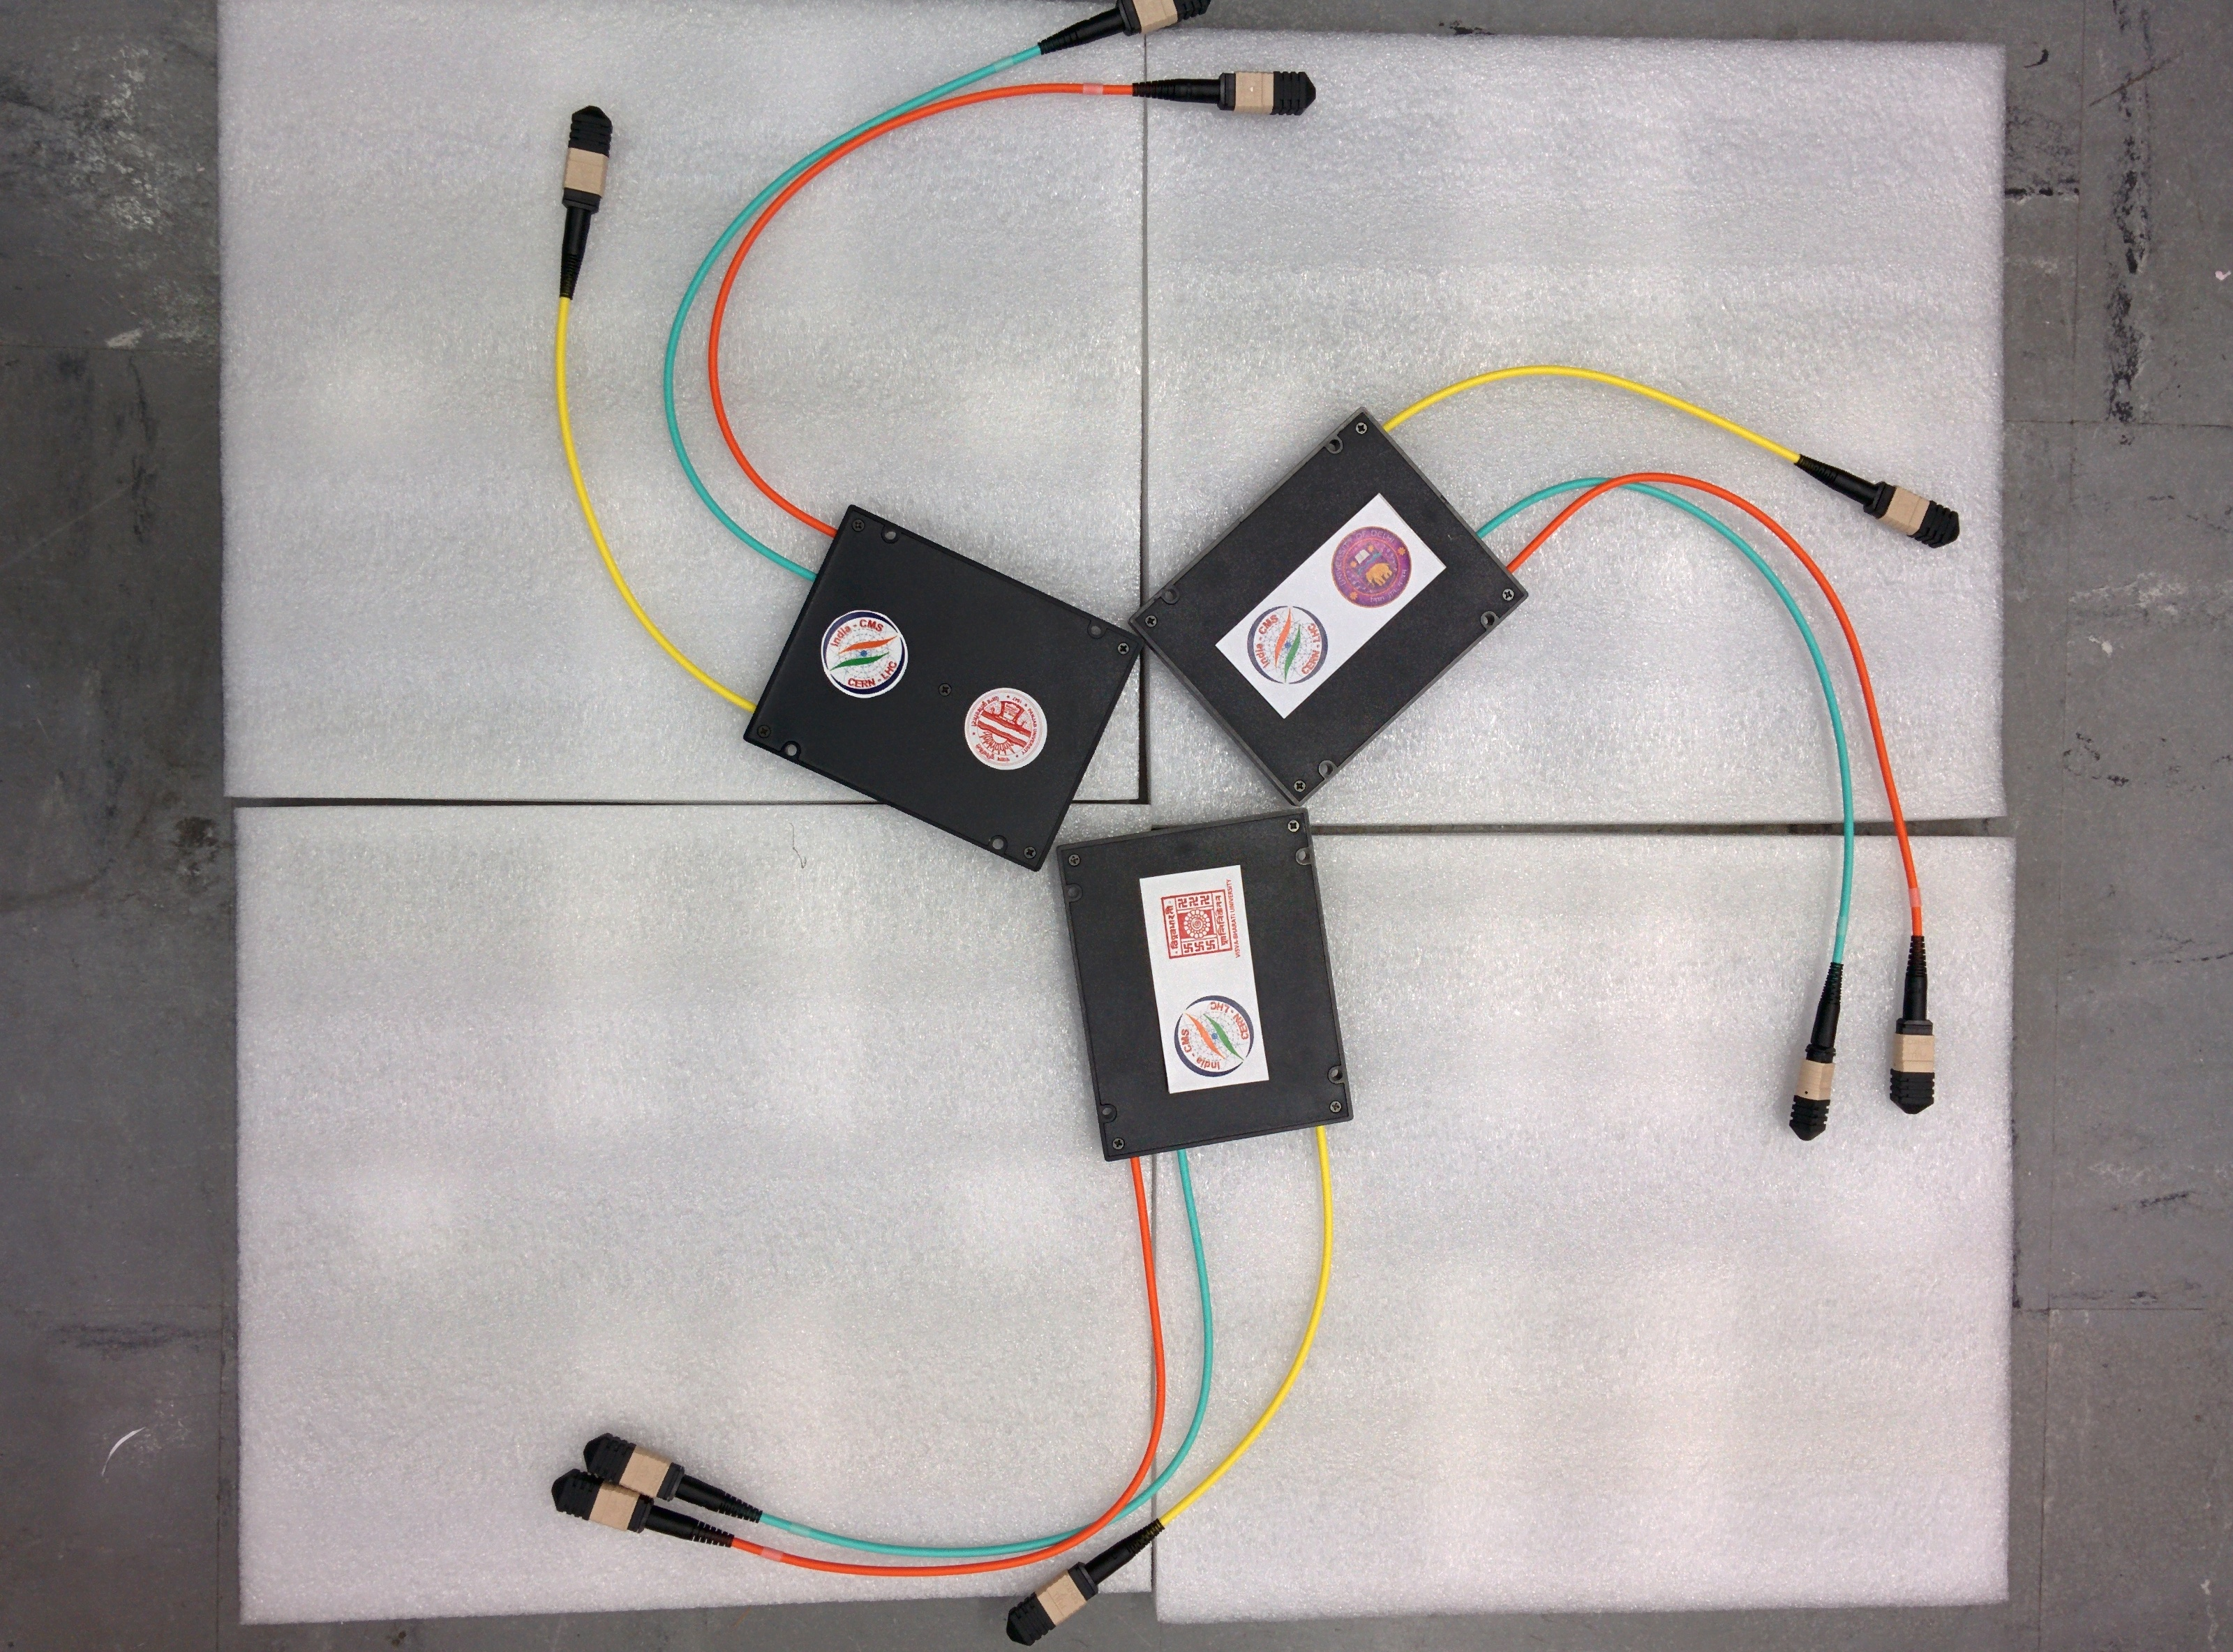
\includegraphics[scale = 0.13]{/home/anter/Desktop/DIS/Presentation/Plots/Triple/4.png}}
\end{overpic}\\
\end{minipage}
\hspace{2mm}
\begin{minipage}[thbp]{0.3\textwidth}
\vspace{-3mm}
\begin{overpic}[scale = 0.16]{/home/anter/Desktop/DIS/Presentation/Plots/CMS-SMP-16-011_Figure_007-c.pdf}%
\put(42,52){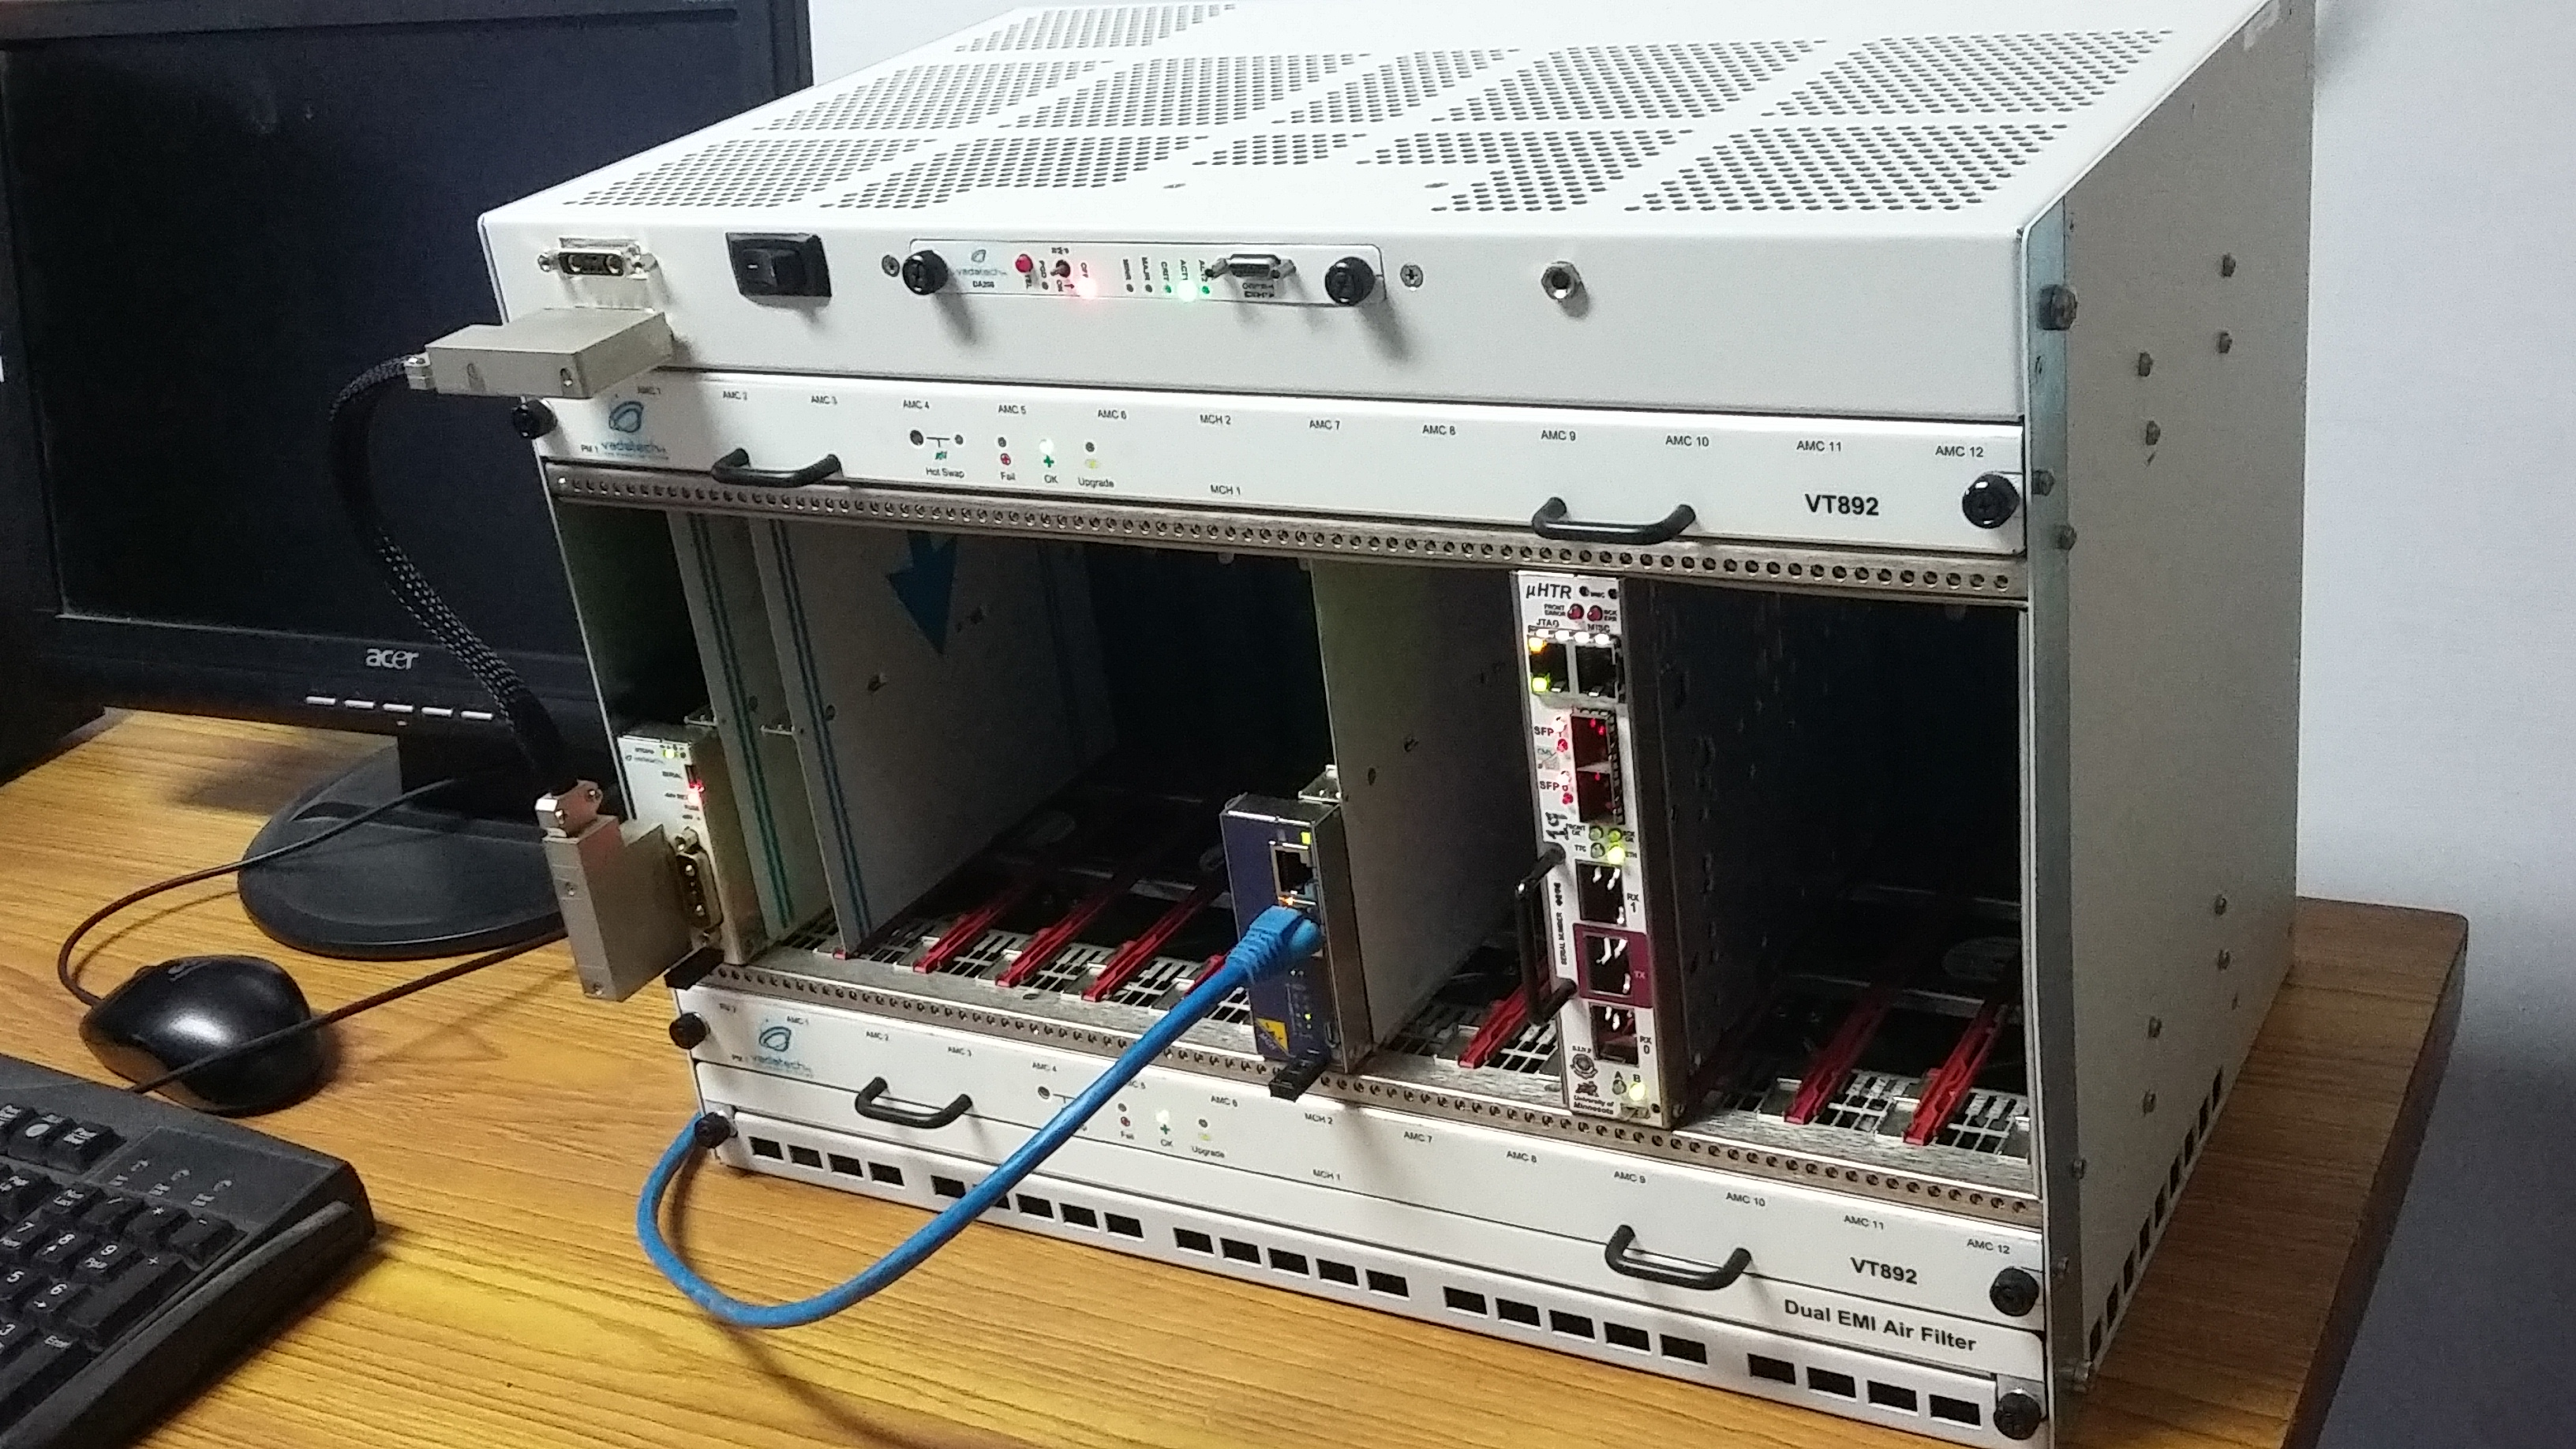
\includegraphics[scale = 0.13]{/home/anter/Desktop/DIS/Presentation/Plots/Triple/1.png}}
\end{overpic}\\
\begin{overpic}[scale = 0.16]{/home/anter/Desktop/DIS/Presentation/Plots/CMS-SMP-16-011_Figure_007-b.pdf}%
\put(42,49){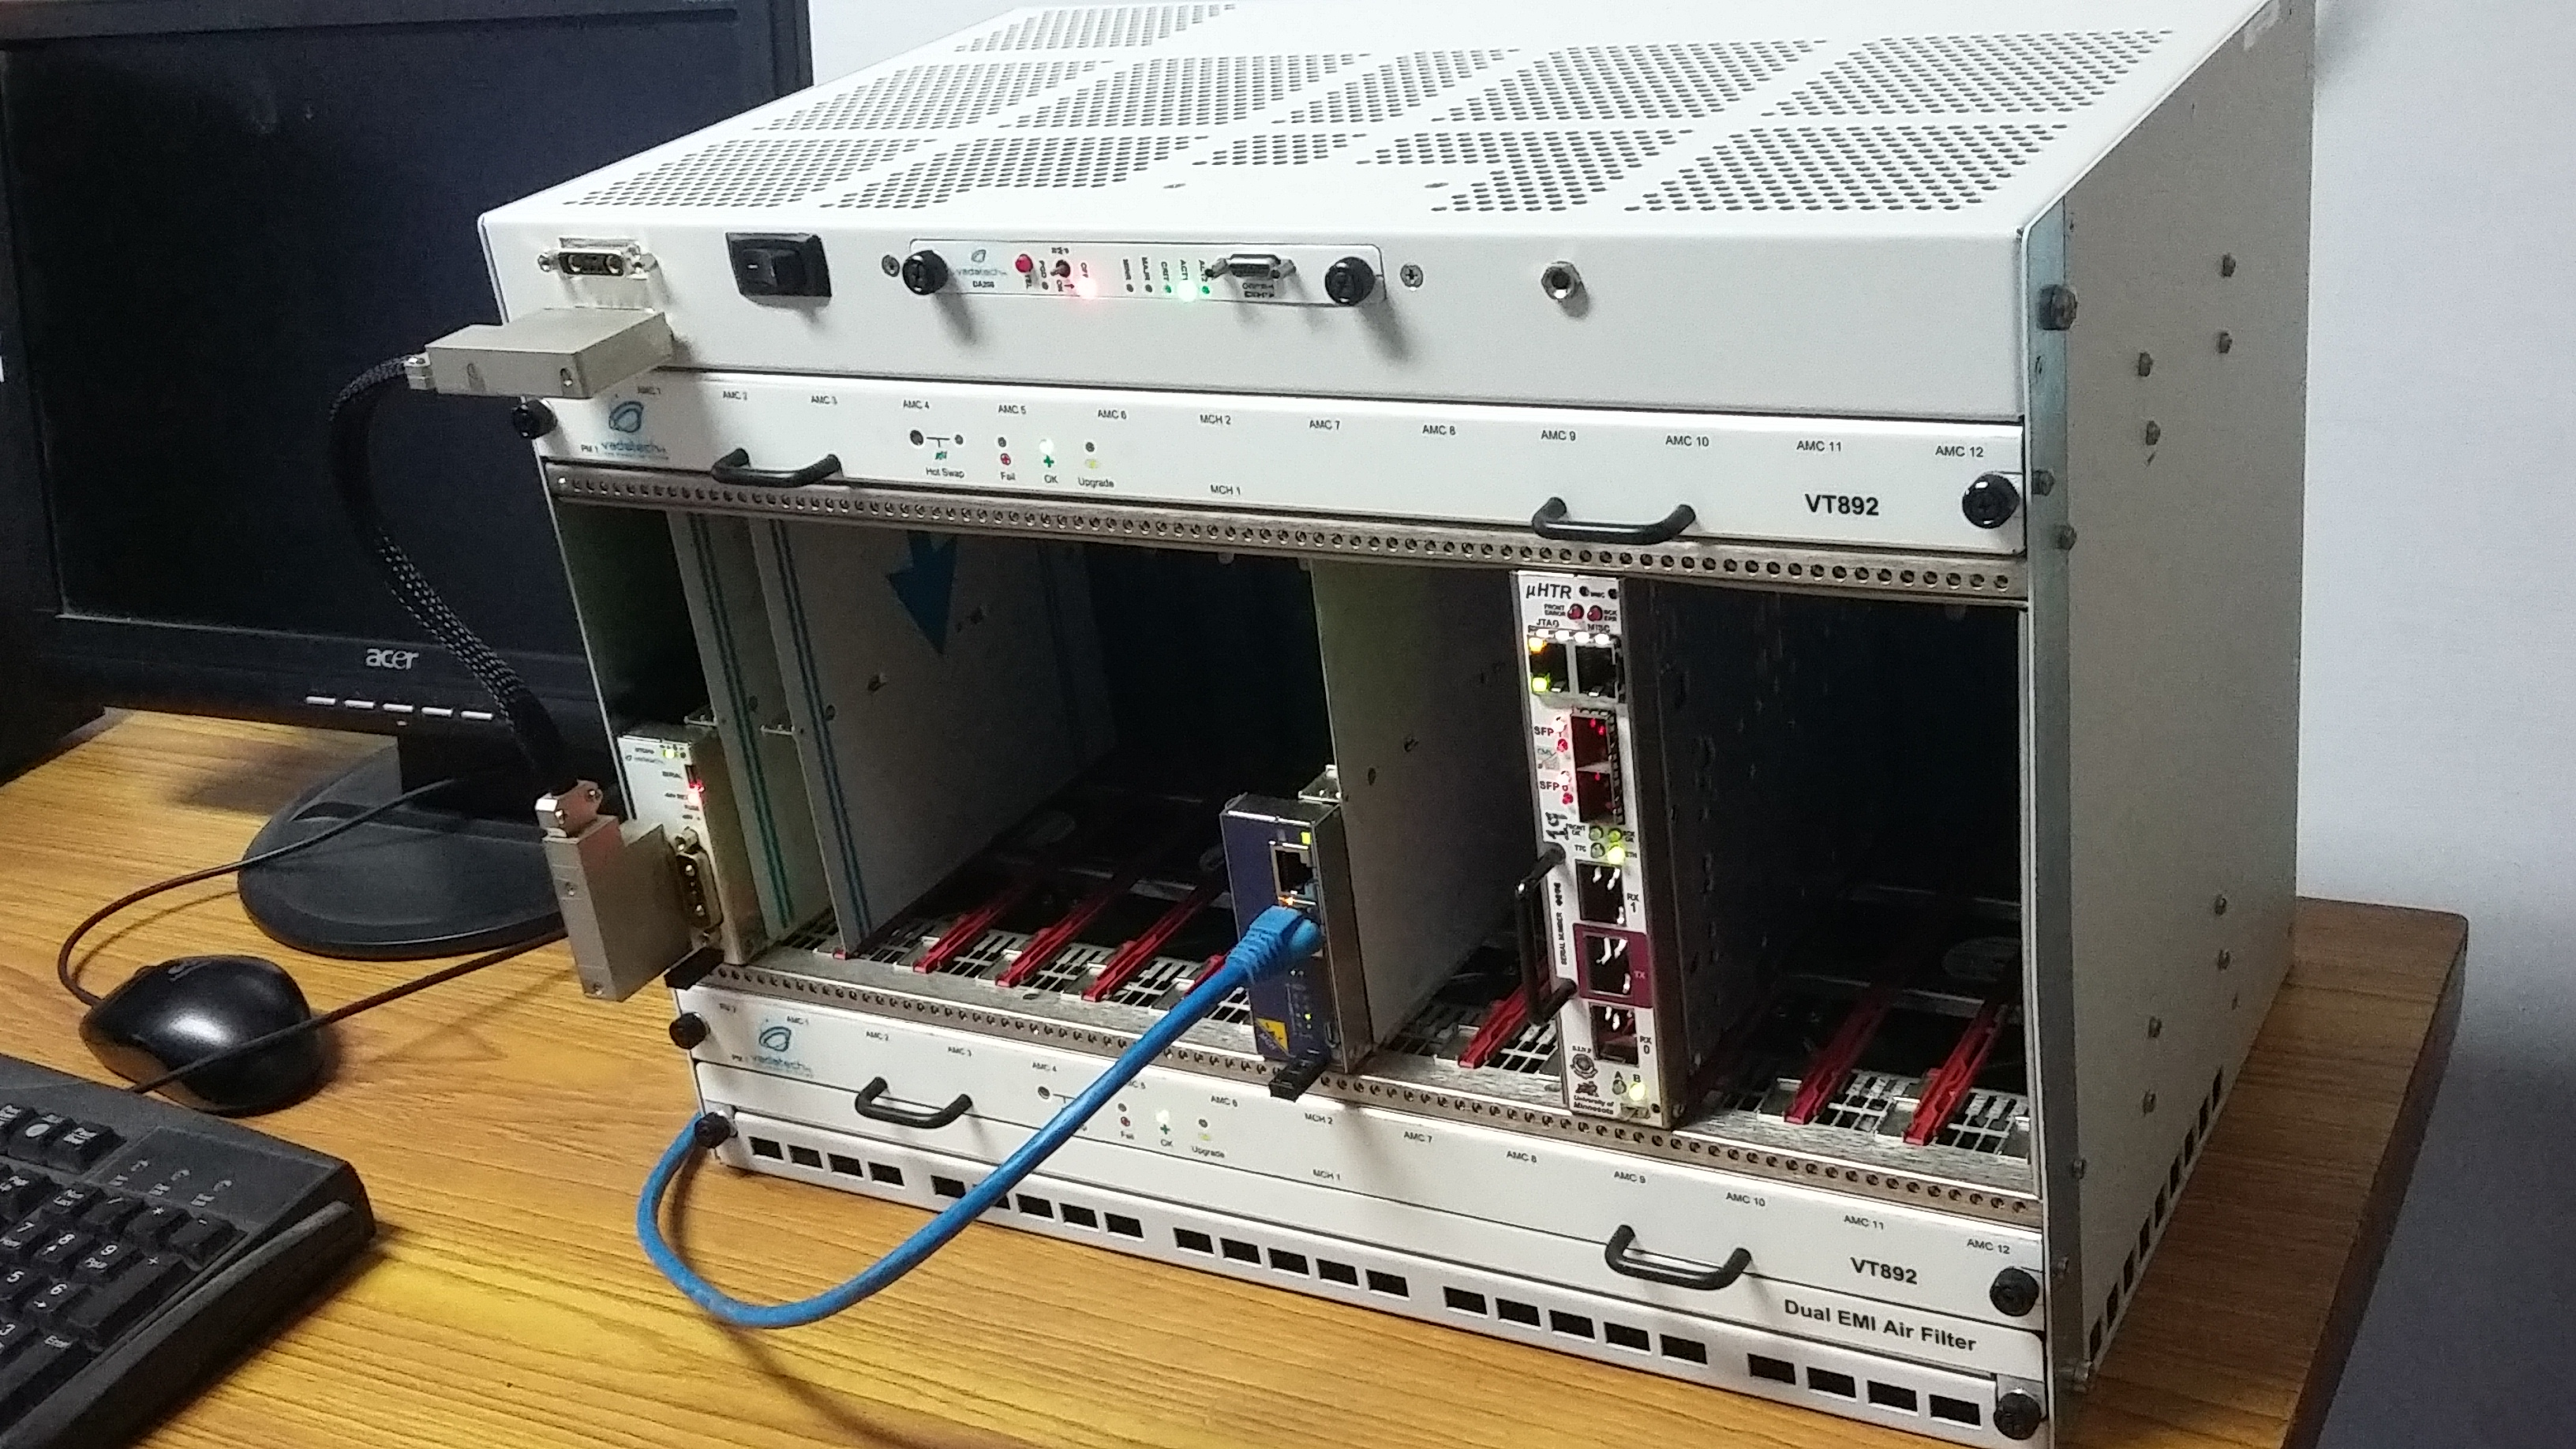
\includegraphics[scale = 0.13]{/home/anter/Desktop/DIS/Presentation/Plots/Triple/2.png}}
\end{overpic}\\
\hspace*{15mm}\begin{beamercolorbox}[wd=23mm,ht=1mm,center,shadow=true, rounded=true]{redgrey}
{}
{\scalebox {0.61} {\mycolor{EPJC 77 (2017) 746}}}
\end{beamercolorbox}
\end{minipage}
\end{frame}

%###################################### Slide : 12 ######################################
\begin{frame}
\frametitle{\centerline{Triple-Differential dijets}}
\setlength\labelsep {\dimexpr\labelsep + 0.05em\relax}
\setlength\leftmargini{\dimexpr\leftmargini + 0.05em\relax}
\hspace*{2mm}\begin{minipage}[thbp]{0.55\textwidth}
\vspace{4mm}
\begin{itemize}
\item {\footnotesize Data are well described in most of the analysed phase spaces. 
\vspace{2mm}
\item Differences observed at high $p_{\rm T,avg}$ and $y_{b}$ : \blue{less known high $x$ region of the PDFs is probed}.
\vspace{2mm}
\item Smaller data uncertainties : \blue{potential to constrain the PDFs.}\\}
\end{itemize}
\vspace{0mm}
\hspace{10mm}\begin{overpic}[scale = 0.16]{/home/anter/Desktop/DIS/Presentation/Plots/CMS-SMP-16-011_Figure_007-d.pdf}%
\put(42,47){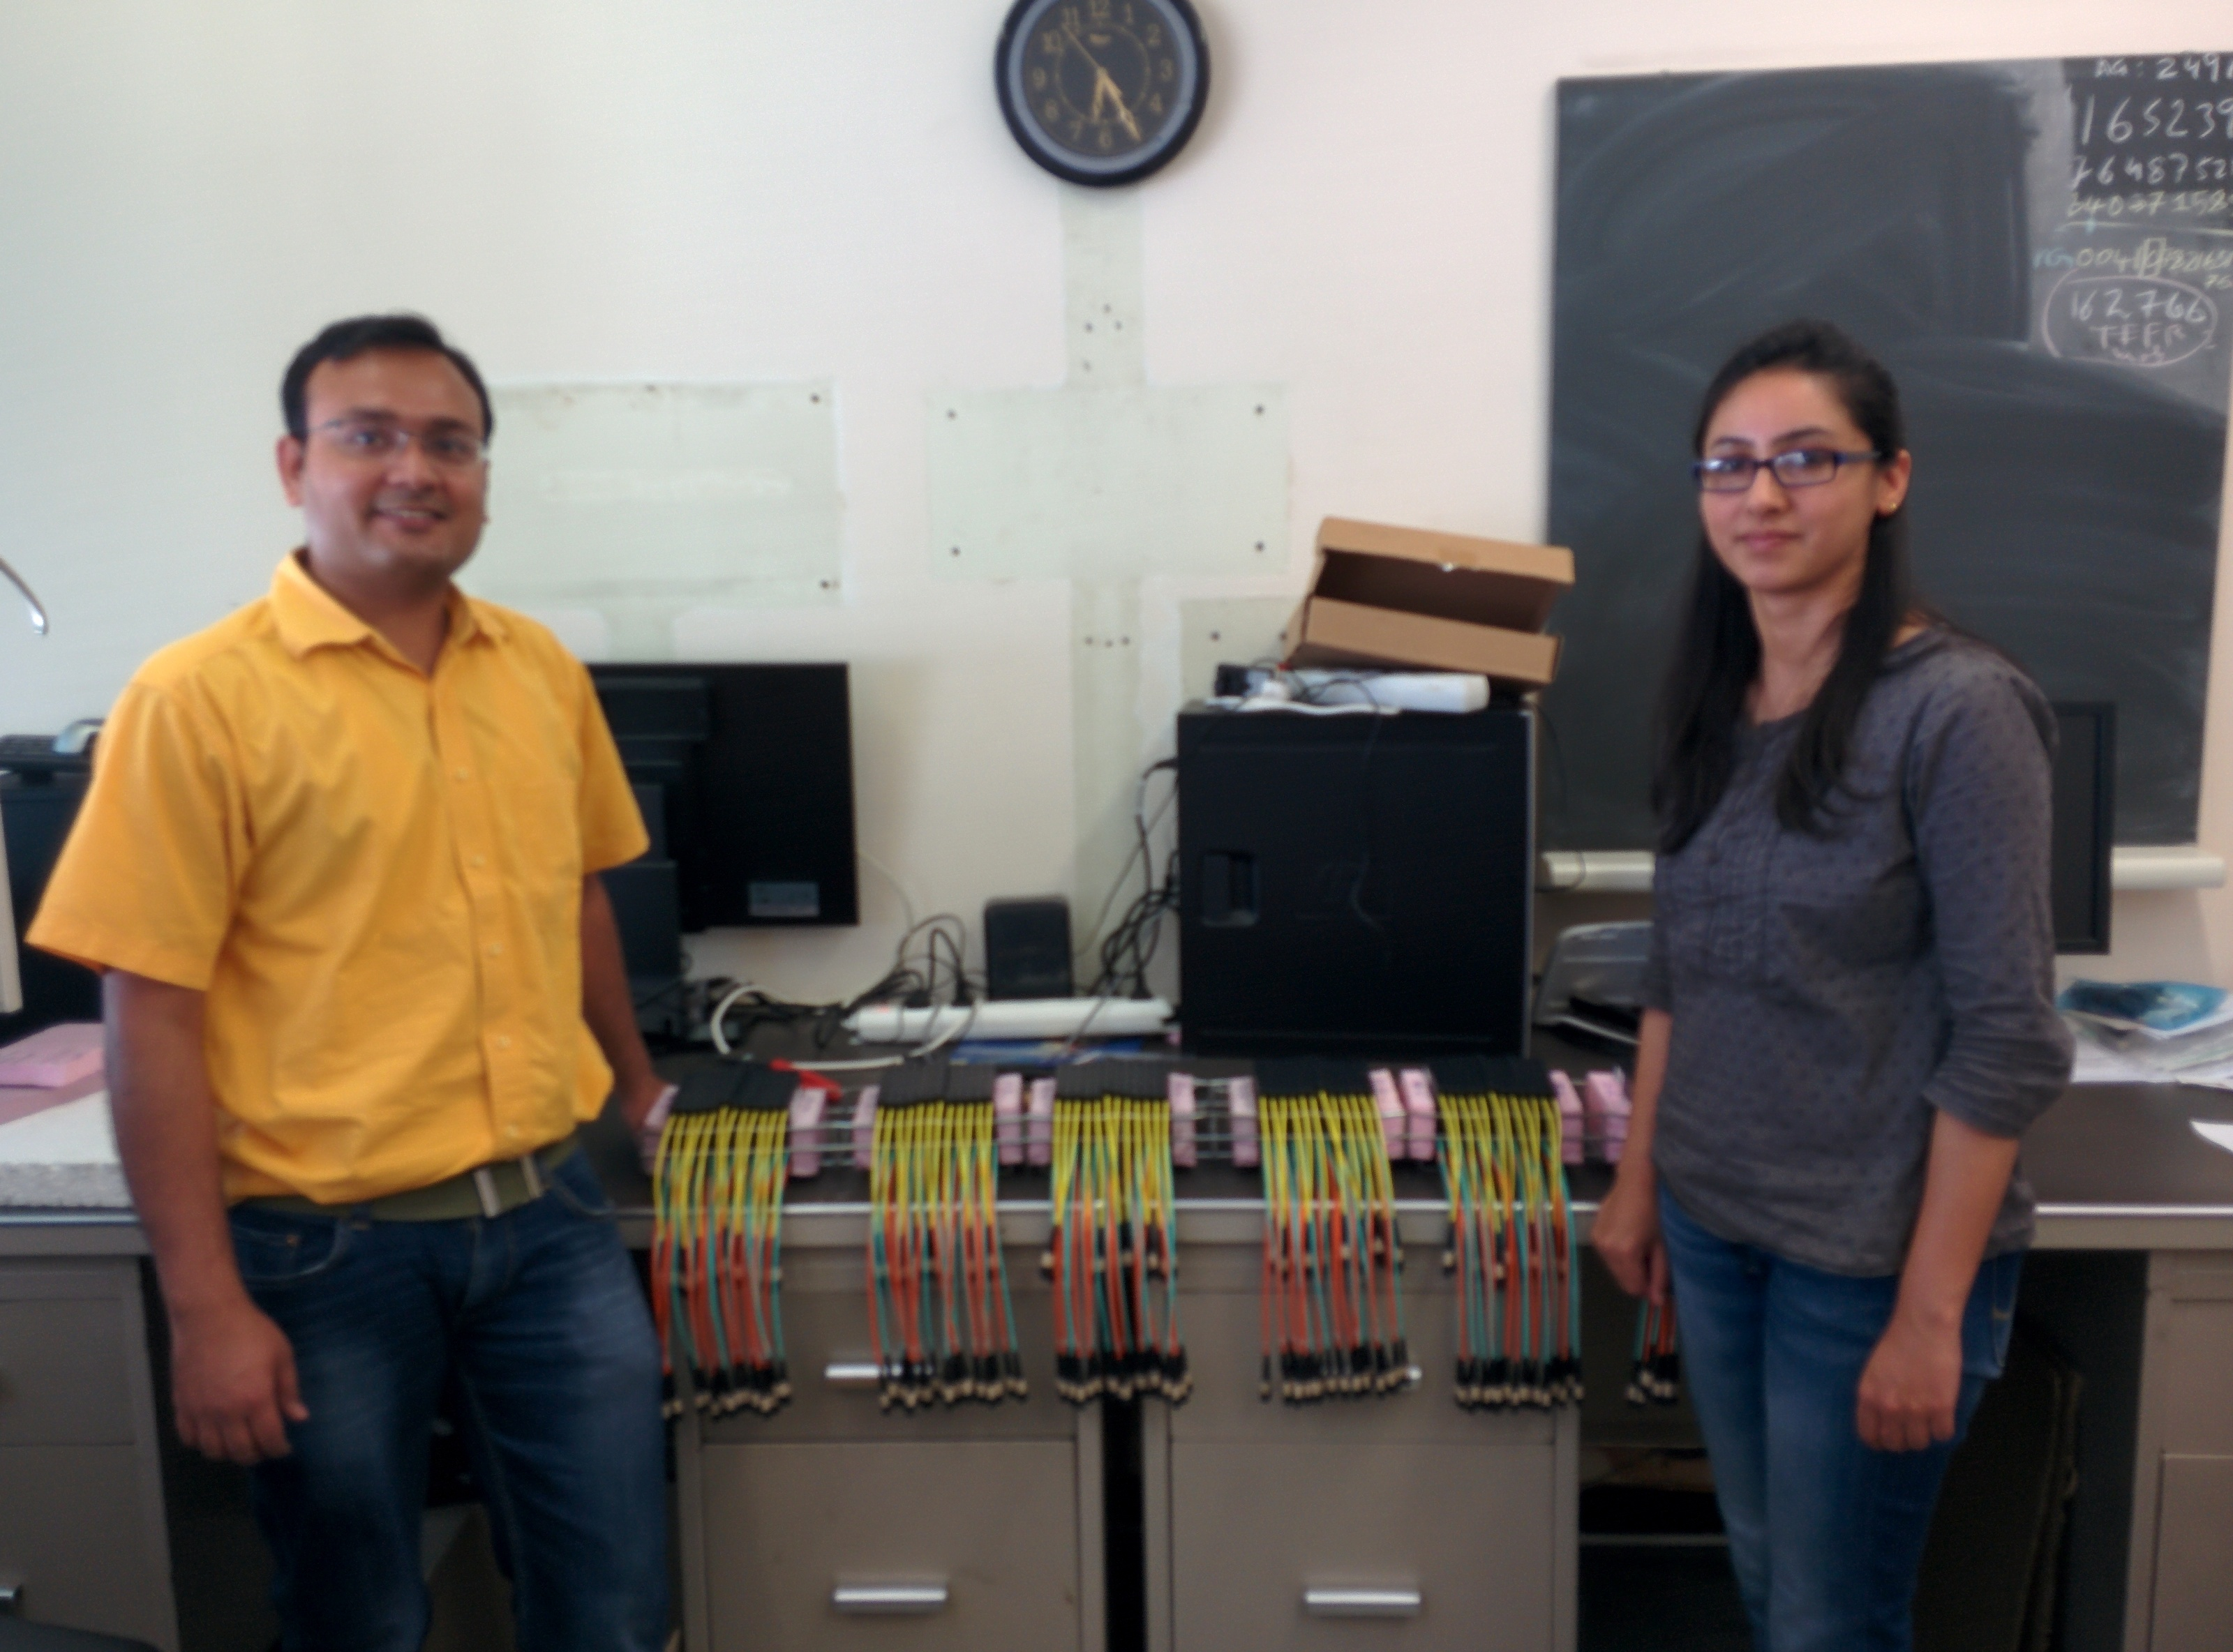
\includegraphics[scale = 0.13]{/home/anter/Desktop/DIS/Presentation/Plots/Triple/5.png}}
\end{overpic}\\
\end{minipage}
\hspace{2mm}
%\vspace{-1.5mm}
\begin{minipage}[thbp]{0.3\textwidth}
\begin{overpic}[scale = 0.16]{/home/anter/Desktop/DIS/Presentation/Plots/CMS-SMP-16-011_Figure_007-e.pdf}%
\put(42,52){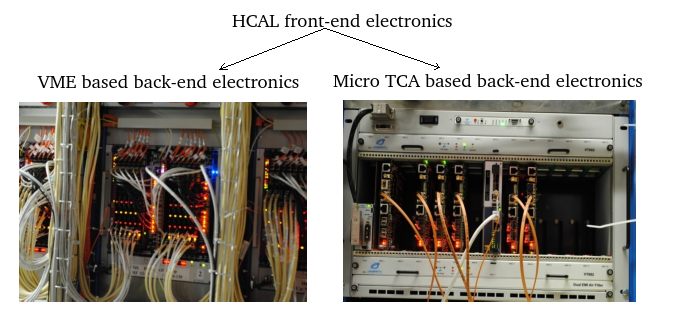
\includegraphics[scale = 0.13]{/home/anter/Desktop/DIS/Presentation/Plots/Triple/3.png}}
\end{overpic}\\
\begin{overpic}[scale = 0.16]{/home/anter/Desktop/DIS/Presentation/Plots/edited_CMS-SMP-16-011_Figure_007-f.pdf}%
\put(42,49){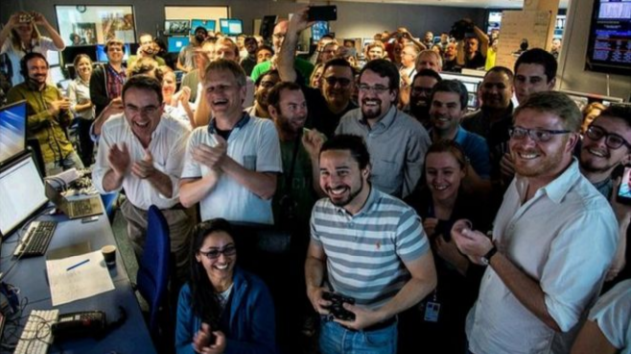
\includegraphics[scale = 0.13]{/home/anter/Desktop/DIS/Presentation/Plots/Triple/6.png}}
%\put(-15,118){\color{red!80!black}\vector(3,-2){108}}
%\put(87,45){\color{red!80!black}\circle{25}}
%{\textcolor{red!80!black}{\solidcirc[10,0]{0.5pt}{0.3}{0.5}}}
\end{overpic}\\
\hspace*{15mm}\begin{beamercolorbox}[wd=23mm,ht=1mm,center,shadow=true, rounded=true]{redgrey}
{}
{\scalebox {0.61} {\mycolor{EPJC 77 (2017) 746}}}
\end{beamercolorbox}
\end{minipage}
\end{frame}

%###################################### Slide : 13 ######################################
\begin{frame}
\frametitle{\centerline{Triple-Differential dijets}}
\setlength\labelsep {\dimexpr\labelsep + 0.05em\relax}
\setlength\leftmargini{\dimexpr\leftmargini + 0.05em\relax}
\hspace*{2mm}\begin{minipage}[thbp]{0.55\textwidth}
\vspace{0mm}
\hspace*{-4mm}\blue{\bf \footnotesize QCD analysis using XFitter (1.2.2)\\}
\vspace{-4mm}
\begin{itemize}
\item {\footnotesize Dijet cross sections \plus HERA inclusive DIS : \\}
\begin{itemize}
\tri
\item {\footnotesize an increased gluon PDF at high $x$ with reduced uncertainties of the PDFs
\vspace{1mm} 
\item change in shape especially at low $Q^2$ \\}
\end{itemize}
\ball 
\item {\footnotesize Comparison of gluon PDFs with inclusive jet data : \\}
\begin{itemize}
\tri
\item {\footnotesize similar shapes of the PDFs and the uncertainties \\}
\end{itemize}
\ball
\item {\footnotesize Precise \alps extraction together with PDF fit : \\}
\end{itemize}
\vspace{2mm}
\hspace*{-3mm}{\scalebox {0.90} {\blue {\alpsmz = 0.1199 $\pm$ 0.0015(exp) $^{+0.0031}_{-0.0020}$(theo)}}}
\vspace{-1mm}
\begin{itemize}
\item {\footnotesize Agreement with the world average value : \\} \vspace{1mm}\hspace*{5mm}{\scalebox {0.90} {\blue{\alpsmz = 0.1181 $\pm$ 0.0011}}}
\end{itemize}
\end{minipage}
\hspace{2mm}
\vspace{1mm}
\begin{minipage}[thbp]{0.3\textwidth}
\includegraphics[scale = 0.16]{/home/anter/Desktop/DIS/Presentation/Plots/CMS-SMP-16-011_Figure_009-a.pdf}\\
\includegraphics[scale = 0.16]{/home/anter/Desktop/DIS/Presentation/Plots/CMS-SMP-16-011_Figure_011-a.pdf}\\
\hspace*{18mm}\begin{beamercolorbox}[wd=23mm,ht=1mm,center,shadow=true, rounded=true]{redgrey}
{}
{\scalebox {0.61} {\mycolor{EPJC 77 (2017) 746}}}
\end{beamercolorbox}
\end{minipage}
\end{frame}

%###################################### Slide : 14 ######################################
\begin{frame}
\frametitle{\centerline{Inclusive multijets}}
\setlength\labelsep {\dimexpr\labelsep + 0.05em\relax}
\setlength\leftmargini{\dimexpr\leftmargini + 0.05em\relax}
\hspace*{2mm}\begin{minipage}[thbp]{0.55\textwidth}
\hspace*{0mm}\begin{beamercolorbox}[wd=52mm,ht=7.0mm,center,shadow=true, rounded=true]{redgrey}
{}
{{\scriptsize \mycolor{\vspace{1mm}Differential cross-section}\\}
\resizebox{0.87\hsize}{!}{$\mycolor{\frac{d\sigma}{d(\httwons)} = \frac{1}{\epsilon~\mathcal{L}_{\mathrm{int,eff}}}\frac{N_\mathrm{event}}{\Delta\big(\httwons\big)}}$}}
\end{beamercolorbox}\\
\vspace{-1mm}
\begin{itemize}
\item {\footnotesize Measurement at 8 TeV, \lumi = 19.7 \inv{fb} 
\vspace{2mm}
\item anti-\kt jets with R = 0.7
\vspace{2mm}
\item {\bf 2-jet and 3-jet event cross sections \\ as a function of : \\ \vspace{2mm}\hspace{6mm}\blue{\httwo = $\frac{1}{2}(p_{\rm T,1}~\plusn~ p_{\rm T,2})$}} 
\vspace{2mm}
\item Theoretical NLO calculations : \\}
\begin{itemize}
\tri
\item {\footnotesize using CT10 PDF set
\vspace{2mm}
\item corrected for non-perturbative (NP) and electroweak (EWK) effects \\}
\end{itemize}
\ball
%\item {\footnotesize Data are well described by theory predictions within uncertainty. \\}
\end{itemize}
\end{minipage}
\begin{minipage}[thbp]{0.3\textwidth}
\vspace*{20mm}
\hspace*{-7mm}\begin{overpic}[scale = 0.3]{/home/anter/Desktop/DIS/Presentation/Plots/CMS-PAS-SMP-16-008_Figure_005-a.pdf}\\
\put(52,42){\mycolor{\bf {\scriptsize 2-jet}}}
%\put(70,43.5){\color{red!80!black}\vector(3,0){30}}
\put(40,29){\green{\bf {\scriptsize 3-jet}}}
%\put(50,22){\color{green!60!black}\vector(0,-1){30}}
\end{overpic}\\\\
\vspace*{-4mm}
\hspace*{25mm}\begin{beamercolorbox}[wd=23mm,ht=1mm,center,shadow=true, rounded=true]{redgrey}
{}
{\scalebox {0.61} {\mycolor{CMS-PAS-SMP-16-008}}}
\end{beamercolorbox}
\end{minipage}
\end{frame}

%###################################### Slide : 15 ######################################
\begin{frame}
\frametitle{\centerline{Inclusive multijets}}
\setlength\labelsep {\dimexpr\labelsep + 0.05em\relax}
\setlength\leftmargini{\dimexpr\leftmargini + 0.05em\relax}
\hspace*{2mm}\begin{minipage}[thbp]{0.56\textwidth}
\vspace{0mm}
\hspace*{-4mm}\blue{\bf \scriptsize Multijet cross sections \\}
\vspace{-4mm}
\begin{itemize}
\item {\scriptsize Data are well described by theory predictions within uncertainty.
\vspace{1mm}
\item EWK corrections explain the increasing excess of the 2-jet data w.r.t. theory ($\sim$1 TeV). \\}
\end{itemize}
\vspace{-0.5mm}
\hspace*{-4mm}\blue{\bf \scriptsize Cross section ratio\\}
\vspace{-4mm}
\begin{itemize}
%\item {\footnotesize \ratio = $\frac{\sigma_{3-jet}}{\sigma_{2-jet}}~\sim$ \alps 
%\vspace{1mm}
%\item Many uncertainties cancel and \blue{sensitive to \alps} \\}
\item {\scriptsize \ratio = $\frac{\sigma_{\rm 3\hy jet}}{\sigma_{\rm 2\hy jet}}~\sim$ \alps
\item Experimental uncertainties, theory uncertainties due to NP effects, PDFs, scale choice, EWK corrections may cancel partially or fully
\item Better tool to extract \alps \\}
\end{itemize}
\vspace{1mm}\hspace{15mm}
\begin{overpic}[scale = 0.20]{/home/anter/Desktop/DIS/Presentation/Plots/CMS-PAS-SMP-16-008_Figure_008.pdf}
\put(22,50){\mycolor{\bf {\scriptsize \ratio}}}
\end{overpic}\\
\end{minipage}
\hspace*{0mm}
\begin{minipage}[thbp]{0.3\textwidth}
\vspace{-4mm}
\begin{overpic}[scale = 0.24]{/home/anter/Desktop/DIS/Presentation/Plots/CMS-PAS-SMP-16-008_Figure_006-a.pdf}\\
\put(22,52){\mycolor{\scriptsize 2-jet}}
\end{overpic}\\
\begin{overpic}[scale = 0.24]{/home/anter/Desktop/DIS/Presentation/Plots/CMS-PAS-SMP-16-008_Figure_006-b.pdf}\\
\put(22,52){\green{\scriptsize 3-jet}}
\end{overpic}\\
\vspace*{-4mm}
\hspace*{20mm}\begin{beamercolorbox}[wd=23mm,ht=1mm,center,shadow=true, rounded=true]{redgrey}
{}
{\scalebox {0.61} {\mycolor{CMS-PAS-SMP-16-008}}}
\end{beamercolorbox}
\end{minipage}
\end{frame}

%###################################### Slide : 16 ######################################
\begin{frame}
\frametitle{\centerline{Inclusive multijets}}
\label{alpha}
\setlength\labelsep {\dimexpr\labelsep + 0.05em\relax}
\setlength\leftmargini{\dimexpr\leftmargini + 0.05em\relax}
%\hspace*{2mm}\begin{minipage}[thbp]{0.7\textwidth}
\vspace*{-0.5mm}
\blue{\bf \scriptsize Determination of \alps\\}
\vspace{0mm}
\begin{itemize}
\item {\scriptsize By minimizing the \chsq between the measurement and the theory
\vspace{0.8mm}
\item In a fit to \rations, using the MSTW2008 PDF set :} {\scalebox {0.59} {\blue {\alpsmz = 0.1150 $\pm$ 0.0023(all except scale) $^{+0.0050}_{-0.0000}$(scale)}}}
\end{itemize}
\vspace{0mm}
%\hspace*{-3mm}{\scalebox {0.58} {$\rm {\bf {\blue {\alpsmz = 0.1150\,\pm0.0010\,\textrm{(exp)}\,\pm0.0013\,\textrm{(PDF)}\,\pm0.0015\,\textrm{(NP)}\,^{+0.0050}_{-0.0000}\,\textrm{(scale)}}}}$}}
%\hspace*{0mm}{\scalebox {0.7} {\blue {\alpsmz = 0.1150 $\pm$ 0.0023(all except scale) $^{+0.0050}_{-0.0000}$(scale)}}}
\begin{itemize}
\item {\scriptsize \alpsmz extracted in ranges of \httwo $\rightarrow$ evolved to \alpsq \\}
\end{itemize}
%\end{minipage}
%\end{minipage}
%\begin{minipage}[h]{0.23\textwidth}

\begin{center}
\vspace{-1mm}
\includegraphics[scale = 0.44]{/home/anter/Desktop/DIS/Presentation/Plots/cropped_CMS-PAS-SMP-16-008_Figure_012.pdf}
\end{center}
%\hspace*{25pt}\begin{beamercolorbox}[wd=23mm,ht=1mm,center,shadow=true, rounded=true]{redgrey}
%{}
%{\scalebox {0.61} {\mycolor{$\alpha_S^{PDG}$ = 0.1181$\pm$0.0011 \\}}}
%\end{beamercolorbox}
%\end{minipage}
\end{frame}

%###################################### Slide : 17 ######################################
\begin{frame}
\frametitle{\centerline{Azimuthal correlations}}
\setlength\labelsep {\dimexpr\labelsep + 0.05em\relax}
\setlength\leftmargini{\dimexpr\leftmargini + 0.05em\relax}
\hspace*{2mm}\begin{minipage}[thbp]{0.73\textwidth}
\vspace{0mm}
\hspace*{0mm}\begin{beamercolorbox}[wd=52mm,ht=7.0mm,center,shadow=true, rounded=true]{redgrey}
{}
{{\scriptsize \mycolor{\vspace{1mm}Normalized differential cross-section}\\}
\resizebox{.97\hsize}{!}{$\mycolor{\frac{1}{\sigma}\frac{d\sigma}{d\Delta\phi_{1,2}},~~~ \frac{1}{\sigma}\frac{d\sigma}{d\Delta\phi^{min}_{2j}} \rm{(3\mbox{-}jet~and~4\mbox{-}jet)}}$}}
\end{beamercolorbox}\\
\vspace{-4mm}
\begin{itemize}
\item {\scriptsize Measurement at 13 TeV, \lumi = 35.9 \inv{fb}
\vspace{1mm}
\item anti-\kt jets with R = 0.4
\vspace{1mm}
\item {\bf Normalized cross sections as a function of the :} \\}
\tri
\begin{itemize}
\item {\tiny \blue{\bf azimuthal angular separation} between the two highest leading \ptr jets
\vspace{1mm} 
\item \blue{\bf minimum azimuthal angular separation} between any two of the three or four leading \ptr jets (3$\mbox{-}$jet and 4$\mbox{-}$jet) \\}
\end{itemize}
\ball
\item {\scriptsize Spectrum gets flatter and become more sensitive to parton shower on moving from 2$\mbox{-}$jet to 3$\mbox{-}$jet to 4$\mbox{-}$jet
\vspace{1mm}
\item Best agreement is given by \green{Herwig7}
\vspace{1mm}
\item POWHEG$\mbox{-}$2J gives better results when matched with \blue{Pythia8} than \textcolor{red}{Herwig\plusn\plus}
\vspace{1mm}
\item \textcolor{purple}{POWHEG$\mbox{-}$3J\plusn Pythia8} is generally lower than \blue{POWHEG$\mbox{-}$2J\plusn Pythia8}\\} 
%\vspace{0.5mm}
%\item \blue{An interesting tool to test the theoretical predictions of multijet production processes} \\ }
\vspace{3mm}\hspace{40mm} \begin{beamercolorbox}[wd=38mm,ht=1mm,center,shadow=true, rounded=true]{redgrey}
{}
{\tiny \mycolor{ arXiv:1712.05471 (Submitted to EPJC)}}
\end{beamercolorbox}
\end{itemize}
\end{minipage}
\hspace{-1mm}
\begin{minipage}[thbp]{0.2\textwidth}
\begin{figure}
\vspace{-2mm}
\hspace*{-3mm} \begin{overpic}[scale = 0.21]{/home/anter/Desktop/DIS/Presentation/Plots/cropped_CMS-SMP-16-014_Figure_001.pdf}%
 \linethickness{4pt}
 \put(-24,38){\includegraphics[scale = 0.19]{/home/anter/Desktop/DIS/Talks/Test/2Jet.png}}
 \end{overpic}
\hspace*{0mm}\includegraphics[scale = 0.20]{/home/anter/Desktop/DIS/Presentation/Plots/cropped_CMS-SMP-16-014_Figure_007.pdf} 
 \end{figure}
\end{minipage}
\end{frame}

%###################################### Slide : 18 ######################################
\begin{frame}
\frametitle{\centerline{Azimuthal correlations}}
\setlength\labelsep {\dimexpr\labelsep + 0.05em\relax}
\setlength\leftmargini{\dimexpr\leftmargini + 0.05em\relax}
%\begin{figure}
\vspace{-1mm}
\hspace*{10mm}
\begin{overpic}[scale = 0.28]{/home/anter/Desktop/DIS/Presentation/Plots/cropped_CMS-SMP-16-014_Figure_010.pdf}
\linethickness{4pt}
\put(-24,38){\includegraphics[scale = 0.21]{/home/anter/Desktop/DIS/Talks/Test/3Jet.png}}
\end{overpic}\hspace*{18mm}\begin{overpic}[scale = 0.28]{/home/anter/Desktop/DIS/Presentation/Plots/cropped_CMS-SMP-16-014_Figure_011.pdf}
\linethickness{4pt}
\put(-24,38){\includegraphics[scale = 0.21]{/home/anter/Desktop/DIS/Talks/Test/4Jet.png}}
\end{overpic}
%\end{figure} 
%{\scriptsize {\bf $\Delta\phi^{min}_{2j}$ Distributions :} \\}
\vspace{-1mm}
\begin{itemize}
%\item {\scriptsize 3-jet topologies (star configuration) : maximum of 2$\pi$/3 
%\vspace{0.5mm}
%\item[] 4-jet topologies (cross configuration) : maximum of $\pi$/2
%\vspace{0.5mm}
\item {\scriptsize {\bf Pythia8 (LO)} exhibits small deviations from the $\Delta\phi_{1,2}$ and fails to describe $\Delta\phi^{min}_{2j}$
\vspace{1mm}
\item {\bf Herwig\plusn\plusn} exhibits the largest deviations from the $\Delta\phi_{1,2}$ but provides a reasonable description of the
$\Delta\phi^{min}_{2j}$
\vspace{1mm}
\item {\bf MADGRAPH\plusn Pythia8} provides a good overall description of the measurements except for $\Delta\phi^{min}_{2j}$ in 4-jet case %\\ }
\vspace{1mm}
\item \blue{An interesting tool to test the theoretical predictions of multijet production processes} \\ }
%\vspace{-1mm}\hfill \begin{beamercolorbox}[wd=38mm,ht=1mm,center,shadow=true, rounded=true]{redgrey}
%{}
%{\tiny \mycolor{ arXiv:1712.05471 (Submitted to EPJC)}}
%\end{beamercolorbox}
\end{itemize}
\end{frame}

%###################################### Slide : 19 ######################################
\begin{frame}
\frametitle{\centerline{Summary}}
\setlength\labelsep {\dimexpr\labelsep + 0.05em\relax}
\setlength\leftmargini{\dimexpr\leftmargini + 0.05em\relax}
\begin{center}
\begin{itemize}
\item {\footnotesize Jet production in pp collisions is one of the main phenomenological predictions of pQCD.
\vspace{2mm}
\item Many interesting results from CMS$^{\mycolor{\star}}$, reaching new levels of precision and exploring new regions of phase space : \\}
\tri
\begin{itemize}
\vspace{2mm}
\item {\footnotesize Measurements of differential jet cross sections over a wide range in transverse momenta from inclusive jets to multi-jet final states are presented. 
\vspace{2mm}
\item Compared to theoretical predictions including those matched to parton shower and hadronization.
\vspace{2mm}
\item Impact on the determination of the strong coupling constant \alps as well as on parton density functions (PDFs) are reported. \\}
\end{itemize}
\ball
\vspace{2mm}
\item {\footnotesize Wide range of jet measurements at various collision energies improve our understanding of QCD. \\}
\end{itemize}
\vspace{4mm}
\hspace*{80mm}\begin{beamercolorbox}[wd=30mm,ht=3.5mm,center,shadow=true, rounded=true]{redgrey}
{}
{\scalebox {0.7} {\mycolor{\LARGE{\bf THANKS!!}}}}
\end{beamercolorbox}
\end{center}
\vspace{-2mm}
{\tiny \mycolor{$^\star$}\url{http://cms-results.web.cern.ch/cms-results/public-results/publications/SMP/index.html}}
\end{frame}

%##################################### Slide : 20 ###########################################
\begin{frame}
\begin{center}
\vspace{15mm}
\textbf{\Large\mycolor{Back-Up Slides}}
\end{center}
\end{frame}

%###################################### Slide : 21 ######################################
\begin{frame}
\frametitle{\centerline{Triple-differential dijets}}
\setlength\labelsep {\dimexpr\labelsep + 0.05em\relax}
\setlength\leftmargini{\dimexpr\leftmargini + 0.05em\relax}
\begin{center}
\includegraphics[scale = 0.12]{/home/anter/Desktop/DIS/Presentation/Plots/CMS-SMP-16-011_Figure_002-a.pdf}%
\includegraphics[scale = 0.12]{/home/anter/Desktop/DIS/Presentation/Plots/CMS-SMP-16-011_Figure_002-b.pdf}%
\includegraphics[scale = 0.12]{/home/anter/Desktop/DIS/Presentation/Plots/CMS-SMP-16-011_Figure_002-c.pdf}\\
\includegraphics[scale = 0.12]{/home/anter/Desktop/DIS/Presentation/Plots/CMS-SMP-16-011_Figure_002-d.pdf}%
\includegraphics[scale = 0.12]{/home/anter/Desktop/DIS/Presentation/Plots/CMS-SMP-16-011_Figure_002-e.pdf}%
\includegraphics[scale = 0.12]{/home/anter/Desktop/DIS/Presentation/Plots/CMS-SMP-16-011_Figure_002-f.pdf}
\vspace{1mm}
\begin{beamercolorbox}[wd=23mm,ht=1mm,center,shadow=true, rounded=true]{redgrey}
{}
{\scalebox {0.61} {\mycolor{EPJC 77 (2017) 746}}}
\end{beamercolorbox}
\end{center}
\end{frame}

%###################################### Slide : 22 ######################################
\begin{frame}
\frametitle{\centerline{Triple-differential dijets}}
\setlength\labelsep {\dimexpr\labelsep + 0.05em\relax}
\setlength\leftmargini{\dimexpr\leftmargini + 0.05em\relax}
\begin{center}
\includegraphics[scale = 0.4]{/home/anter/Desktop/DIS/Presentation/Plots/CMS-SMP-16-011_Table_002.pdf}\\
\vspace{3mm}
\hspace{10mm}\begin{beamercolorbox}[wd=23mm,ht=1mm,center,shadow=true, rounded=true]{redgrey}
{}
{\scalebox {0.61} {\mycolor{EPJC 77 (2017) 746}}}
\end{beamercolorbox}
\end{center}
\end{frame}

%###################################### Slide : 23 ######################################
\begin{frame}
\frametitle{\centerline{Triple-differential dijets}}
\setlength\labelsep {\dimexpr\labelsep + 0.05em\relax}
\setlength\leftmargini{\dimexpr\leftmargini + 0.05em\relax}
\begin{center}
\includegraphics[scale = 0.3]{/home/anter/Desktop/DIS/Presentation/Plots/CMS-SMP-16-011_Figure_010.pdf}\\
\vspace{0mm}
\hspace{10mm}\begin{beamercolorbox}[wd=23mm,ht=1mm,center,shadow=true, rounded=true]{redgrey}
{}
{\scalebox {0.61} {\mycolor{EPJC 77 (2017) 746}}}
\end{beamercolorbox}
\end{center}
\end{frame}

\end{document}
